%!TEX options = --shell-escape

\documentclass[master]{thesis-uestc}
\usepackage{minted}
% \usepackage[utf8]{inputenc}
\usepackage{verbatim}
% Default fixed font does not support bold face
\DeclareFixedFont{\ttb}{T1}{txtt}{bx}{n}{09} % for bold
\DeclareFixedFont{\ttm}{T1}{txtt}{m}{n}{09}  % for normal

% Custom colors
\usepackage{color}
\definecolor{deepblue}{rgb}{0,0,0.5}
\definecolor{deepred}{rgb}{0.6,0,0}
\definecolor{deepgreen}{rgb}{0,0.5,0}

\usepackage{listings}
\usepackage{amsmath}
\usepackage{fancynum}
\usepackage[nottoc]{tocbibind}

% \usepackage{listings}

% \title{REAL-TIME FACIAL EMOTION RECOGNITION RESEARCH BASED ON DEEP LEARNING AND AN APPLICATION FRAMEWORK IMPLEMENTATION}

% \author{BAFFOUR ADU ASARE}

% \advisor{PROFESSOR\chinesespace JIANDONG GUO}

% \school{SCHOOL OF INFORMATION AND SOFTWARE ENGINEERING}

% \major{SOFTWARE ENGINEERING}

% \studentid{201724220103} 

\begin{document}
%\makecover
\begin{chineseabstract}
近年来,在人工智能领域,面部表情的识别备受人们的关注。许多研究工作利用具有数百万可训练参数的大型卷积神经网络,最终获得了很高水平的结果。当然这要求计算机拥有很高的计算能力,但是这些深度学习模型对于实时应用是不可行的,尤其是运行在例如移动电话等功率受限的设备上。
在本论文中,为了进行实时的人脸表情识别,我们提出了一种新的、高效的“轻量级”卷积神经网络。我们提出的模型架构是基于深度可分离2D卷积实现的,它可以大大减少网络参数,从而加快整体性能速度,使其对于实时应用是可行的。我们提出的模型中包含的参数总数大约只有400千。该模型的基本操作包括:深度可分离卷积、批量规范化、最大化、全局平均池化和归一化。这些基本操作被周密地组合在一起,创建了一个具有21层的CNN架构。我们通过在FERC-2013数据集,日本女性面部表情(JAFFE)数据库和扩展Cohn-Kanade数据集(CK +)上对该模型进行了测试。该模型获得的FERC-2013数据集的测试精度高达69\%,JAFFE数据集的测试精度高达80\%,CK +数据集的测试精度高达99\%。显而易见的是,我们的模型以很少的参数实现了非常有竞争力的结果,并且为实时应用提供了比最先进模型更好的选择。最后,我们通过将实时视频流连接到面部检测器,以将图像提供给训练的模型,最终证明我们的模型可以满足实时应用的需求。该模型将面部表情分为七种情绪:愤怒,厌恶,恐惧,快乐,中立,悲伤和惊喜。


\chinesekeyword{面部表情识别,深度可分卷积,深度学习,卷积神经网络,实时}
\end{chineseabstract}

\begin{englishabstract}
Facial expression recognition has gained much research interest in the last few years in the field of artificial intelligence. Many research works have achieved state-of-the-art results using large convolutional neural networks containing millions of trainable parameters requiring high computing power. Such deep learning models involve much computation, thus, making them unfeasible for real-time application, especially running on power constrained devices like mobile phones. In this thesis, we propose a new and efficient `lightweight' Convolutional Neural Network for facial emotion recognition in real-time. Our proposed model architecture is based on the implementation of depthwise separable 2D convolution which reduces the network parameters drastically thereby accelerating the overall performance speed making it seemingly feasible for applications in real-time. The total number of parameters contained in our proposed model is about only 400 thousand. The basic operations of the model include: depthwise separable convolution, batch normalization, max-pooing, global average pooling and softmax. These basic operations are carefully put together to create a twenty-one layer CNN architecture. We experiment our model on FERC-2013 dataset, the Japanese Female Facial Expression (JAFFE) database and the Extended Cohn-Kanade Dataset (CK+). Our model obtained test accuracy up to 69\% for FERC-2013 dataset, 88\% for JAFFE dataset and an outstanding 99\% for CK+ dataset. It is evident that our model achieves very competitive results with few parameters and presents itself a better choice over state-of-the-art models for real-time applications. Finally, we demonstrate that our model can meet real-time needs by connecting a live video stream to a face detector to feeding images to our trained model. The model classifies facial expressions into one of the seven emotions (Anger, Disgust, Fear, Happy, Neutral, Sad and Surprise).

\englishkeyword{Facial Emotion recognition, Depthwise Separable Convolution, Deep learning, Convolutional Neural network, Real-time}
\end{englishabstract}

\thesistableofcontents
\thesisfigurelist
\thesistablelist


\thesischapterexordium

In this chapter, the thesis background and the thesis significance will be introduced. The state-of-the-art in this research area will be outlined to give grounds for the contribution and innovation of this thesis. 

\section{Research Background and Significance}
Facial Emotion Recognition (FER) is simply the process of detecting emotions of humans based on their facial expressions. The task of FER is obviously quite easy and natural for a person to solve without effort or delay, regardless of gender, age, race, and even in the presence or absence of eyeglasses, jewelry, mustache or beard\cite{Ivanovsky-2017}. Facial expressions are significant elements in human communication that enables us better comprehend each other's intentions and feelings in communications. According to M. Albert\cite{albert1968}, we have three basic aspects in any confronting communication; namely: words, tone of voice, and nonverbal elements. A survey conducted by M. Albert\cite{albert1968} shows that nonverbal elements conveys two-thirds of human communication whiles verbal (words and tone of voice) conveys one-third of human communication. Some examples of nonverbal communication elements include eye contact, shaking hands, patting the back, hugging, facial expressions, and many more. Furthermore, M. Albert\cite{albert1968} reports that among the several nonverbal communication forms, facial expression contains 55\% of messages pertaining to feelings and attitudes. Due to the rich informative clues in facial expressions, it becomes natural that over the most recent couple of decades, facial emotion recognition has been very much interested to researchers; and its been researched for feasible applications in cognitive science, affective computing and computer animations.

\begin{figure}[ht]
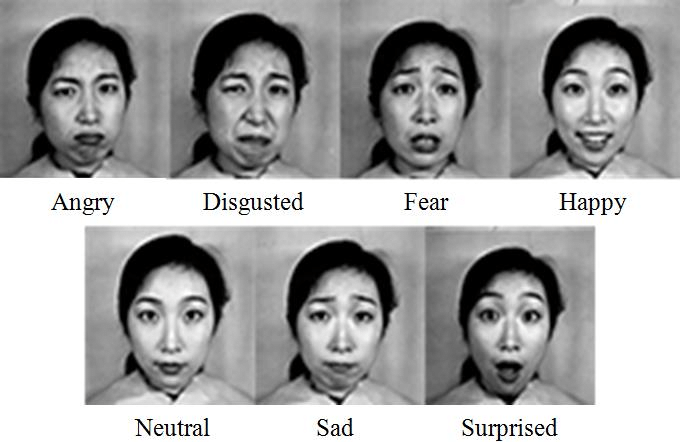
\includegraphics[width=5in]{pic/7_basic_emotions.png}
\caption{\,\,\,\,\,\,\,\,\,\,The seven classes of basic emotions expression. Source: M. Lyons et al.\cite{Michael-2017})}
\label{7_basic_emotions}
\end{figure}

FER can be used and applied in many areas including clinical psychology, medical diagnosis, human computer interaction (for example to analyze the impact of advertisements), forensics (lie detectors) and so on\cite{Ivanovsky-2017, sang-2017}. FER can also be beneficial in robotics, for example if robots are able to predict human emotions, they can be guided by the detected emotion and respond appropriately. In addition, FER in recent years have become popular in video analytic applications, such as evaluating front office staff performance, in security systems of terrorist identification and interrogation\cite{sang-2017}.

In everyday life, the human face expresses a wide range of expressions. Building computer algorithms for FER compels us to identify certain classes of facial expressions. There are seven basic emotions that most research works have focused on, which have become universally accepted in many cultures. There are: neutral, happy, surprise, fear, angry, sad, and disgust\cite{Yu:2013:LRF:2459511.2459661}. Samples of the seven basic expression classes are shown in Figure \ref{7_basic_emotions}. Humans sometimes express other forms of emotions such as compound emotions, i.e. a combination of two basic emotions, e.g. happily surprised, happily sad, sadly fearful, and sadly surprised. Another form of emotion is micro emotions, i.e. impromptu and slight facial actions happening involuntarily. Micro emotion is the type of emotion that shows the honest and hidden emotions of a person exhibited in a short period\cite{josh2018}. Samples of micro emotions are shown in Figure \ref{micro_emotions}.

\begin{figure}[ht]
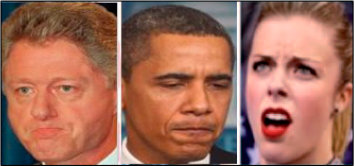
\includegraphics[width=5in]{pic/micro_expressions.png}
\caption{\,\,\,\,\,\,\,\,\,\,Sample examples of spontaneous expressions. Source: D. Joshi\cite{josh2018})}
\label{micro_emotions}
\end{figure}

The task of facial emotion recognition has some challenges. Some of these challenges include: illumination, face pose (rotation), optical obstacles, face blur, noise in image, individual difference of subjects, spontaneous emotion, etc\cite{Ivanovsky-2017, josh2018}. Thus, the task of a FER algorithm must tackle all these challenges and output correct recognition results in real-time. In this order, many different methods have been proposed and studied. These approaches can be grouped into two, namely: Conventional FER approach and Deep-Learning Based FER approach\cite{Ivanovsky-2017}.

Conventional FER approach studies and detects the face region and extracts geometric features, appearance features, or a hybrid of geometric and appearance features from the input face image. Most often, feature extraction in conventional approaches are handcrafted by experts. HoG, LBP, distance and angle relationship between landmarks are popular handcrafted features used to pre-train classifiers, like SVM, AdaBoost, and random forest\cite{Ivanovsky-2017}. Conventional methods use somewhat lower computing power than deep learning-based approaches but very difficult to optimize to achieve real-time performance. This is because feature extraction is done by an expert whiles classifiers are devised by the programmer; joining and optimizing these two processes to increase performance is almost impossible\cite{Ivanovsky-2017}. Additionally, since features are handcrafted, there are overheads of finding the exact features suitable to build and pre-train robust classifiers for FER with environmental factors like illumination, occlusion, noise in image, individual difference of subjects, etc. in mind.

Applying deep learning algorithms like convolutional neural network (CNN) and recurrent neural network (RNN) in the field of computer vision have gained a quantum leap in recent decades. With CNN, it has the ability of automatically learning at full-length the features that are optimal precisely from the input image. Thus, the reliance on physics-based methods and handcrafted features (pre-processing technique) are removed or highly reduced. This is a great advantage compared to conventional approach where the algorithm accuracy depends heavily on handcrafted features. However, deep learning algorithms come with their disadvantages as well. High computing power and memory are required for training the models containing millions of parameters. This setback makes deep learning algorithms impractical for real-time performance.

In the quest to solve this problem more efficiently and accurately, we propose and construct an efficient deep learning model based on depthwise separable convolution. The model is trained with augmented data very close to real world images. We test and deploy our model to recognize the seven basic emotions in real-time.

\section{State of Arts}
The methods proposed over the years for facial emotion recognition can be classified into two groups, namely: Conventional approach and Deep learning based approach.

\subsection{Conventional Approaches}
Conventional approaches for facial emotion recognition perform recognition based on hand-engineered features; commonly by identifying the face region and extracting geometric features, appearance features, or a hybrid of geometric and appearance features.

Ghimire and Lee\cite{ghimire2013} extracted geometric features from video sequences of facial expression images based on the position and angle of 52 facial landmark points. Further processing was done by calculating the Euclidean distance between landmark pairs within a frame; and subtracting the angle and distance from the corresponding distance and angles in the first frame of the video sequence. Two classifiers were presented, using a multi-class AdaBoost algorithm with dynamic time warping gained recognition accuracy of 95.17\%; and using SVM on the boosted features gained recognition accuracy of 97.35\%.

Happy et al.\cite{Happy-2017} extracted appearance features by using local binary pattern (LBP) histogram of different block sizes of a global face region as the feature vectors; the algorithm classified facial expressions into six basic emotions, namely: happiness, sadness, disgust, fear, surprise and anger, using principal component analysis (PCA). The recognition accuracy of the algorithm diminished when implemented in real-time caused by inability to reflect local variations of the facial components to the feature vector. In contrast to global-feature-based approach, different regions of the face have different levels of importance for facial emotion recognition\cite{josh2018}. Ghimire et al.\cite{ghimire2013} extracted region-specific appearance features by dividing the entire face into domain-specific local regions. Important local regions were determined by using incremental search approach which resulted in the reduction of feature dimension and improvement in recognition accuracy.

Some approaches fused geometric and appearance features to balance the weaknesses of the two approaches and achieved even better results in certain cases. Suk and Prabhakaran\cite{MSu14} extracted facial expression features by Active Shape Model(ASM) fitting landmarks on a face and then dynamic features were generated by the displacement between neutral and expression features. The algorithm gained 86\% accuracy in 309 video samples on the extended Cohn-Kanade (CK+) dataset\cite{5543262}. Although, the algorithm was implemented in real-time mobile, the accuracy tends to degrade to about 72\% for six posed basic emotion recognition.

\subsection{Deep Learning based Approaches}
For deep learning methods, especially CNNs, they have gained a breakthrough in image-related problems in recent decades due to the ability to automatically learn and extract good optimal representations directly from the images. Previous works like LeNet-5\cite{YLe98}, AlexNet\cite{Kri12}, VGG-16\cite{Kar14}, GoogleNet\cite{Chr14}, and ResNet\cite{Kai15} have demonstrated the significance and power of CNNs in the field of computer vision.

Rassadin et al.\cite{DBLP:journals/corr/abs-1709-01688} described an algorithm which was used for submissions in the fifth Emotion Recognition in the Wild (EmotiW 2017) group-level emotion recognition sub-challenge. They trained a CNN model for face identification task to extract feature vectors of detected faces rather than pre-training on emotion recognition problems. Then an ensemble of Random Forest classifiers were learned to predict emotion score using available set. If no faces were detected, one member of the ensemble extracts features from the whole image. The method achieved 75.4\% accuracy on the validation data, which is 20\% higher than the handcrafted feature-based baseline.

Ivanovsky et al.\cite{Ivanovsky-2017} presented an algorithm for smile detection and facial expression recognition based on CNN. The model was trained using face images from the CMU Pose, Illumination, and Expression (PIE) database\cite{Sim-2003-8822} and achieved test accuracy of 84.98\% and 94.73\% for smile detection and facial expression recognition respectively. Even though the algorithm is quite simple for its implementation and has good test results, from the architecture of the network, it is evident that the model has large parameters and it requires great computational power; thus, making it impractical for real-time usage. Furthermore, the algorithm often confused facial expression squint for disgust.

Dinh et al.\cite{sang-2017} proposed a so called effective architecture of CNN for facial emotion recognition by applying multi-class SVM loss function. They applied data augmentation techniques to increase the amount of training samples in FERC-2013 dataset\cite{kaggle_ferc} in order to avoid overfitting. The model gained accuracy up to 71.0\% for public test and 71.9\% for private test for seven emotion classes. Consequently, the model exhibits similar drawbacks as observed in the work of Ivanovsky et al.\cite{Ivanovsky-2017} with about 29\% wrongly classified images.

Xiao et al.\cite{8273609} proposed an improved facial emotion recognition method based on region of interest (ROI) to guide the CNN focus on the areas associated with the facial expression. In the test stage, two recognition methods were investigated: (1) recognising the target image directly; and (2) recognising target image by implementing decision fusion strategy on ROI areas.  The performance of the algorithm was validated on augmented CK+ dataset gaining an average test accuracy of 94.53\%. This method outperformed the work done by D. Sang et al.\cite{sang-2017} but suffers (1) higher computational cost to further perform decision fusion on ROI areas (2) high requirement for the distributed representations of the trained model; herein, making it impractical for real time applications. Also, amplifying ROI images to gain details compared with the original image may cause discrimination of the local representation to some extent.

Song et al.\cite{6776135} proposed and trained a model based on CNN that achieved facial emotion recognition in real-time on a smart phone using a client-server architecture. A smart phone captures the user's face, sends request to facial expression recognition server, server takes as input the face image and the trained model predicts the facial emotion expressed (anger, happiness, sadness, surprise or neutral). The server reports back to the smart phone. Despite high training accuracy of 99.2\%, 97.1\%, 95.5\%, and 84.5\% on CK+ dataset, SAIT , SAIT2  and Internet  datasets respectively; and its real-time achievement of about 100ms of round-trip time per image, the model is  not generalized and robust; i.e. no evaluation metrics were provided to assess the model performance and accuracy in real-time.

Chen et al.\cite{7988558} proposed a CNN model for the task of facial emotion recognition that improved the recognition accuracy up to 98.15\%, which is about 4\% higher compared to AlexNet network on the CK+ dataset with the help of adding Batch Normalization (BN) layers to the network. They went further to implement the model in real-time to recognize facial expressions. This method gained higher training accuracy compared to the average training accuracy of Song et al.\cite{6776135}, however, both methods share same drawbacks, that is generalizing and robustness with high computational cost.

Duncan et al.\cite{duncan2016} developed a convolutional neural network for classifying human emotions from dynamic facial expressions in real time. They used transfer learning on the fully-connected layers of VGG's network which was pre-trained for the task of human emotion classification. To improve the model accuracy, they applied transfer learning on the JAFFE\cite{Michael-2017} and CK+ datasets. Their model achieved an overall training accuracy of 90.7\% and test accuracy of 57.1\%. Finally, a live video stream connected to a face detector feeds images to the neural network for real-time facial emotion classification. During training, they applied randomized jitter by randomly changing both cropping (10\% variation) and brightness (20\% variation) in the input images; in order to account for real environment factors such as lighting, distance from the camera, incorrect face cropping, and variations in orientation of the subject face, which are mostly omitted in a laboratory. It can be observed that higher accuracy was achieved (> 90\%) under the laboratory environment with perfect lighting, camera at eye level, subject facing camera with an exaggerated expression but there was significant fall in accuracy (57.1\%) when tested under real environmental conditions.

Jung et al.\cite{7410698} proposed a deep learning network based on two different models of CNN. The first model extracts temporal appearance features from image sequences, whereas the second deep learning network extracts temporal geometry features from temporal facial landmark points. Unlike traditional integration methods like weighted summation and feature concatenation, these two models were combined to cooperate with each other using a new integration method called joint fine-tuning in order to boost the performance of the facial expression recognition. This method achieved accuracy up 97.25\% for CK+ dataset, 81.46\% for Oulu-CASIA dataset\cite{ZHAO2011607}, and 70.24\% for MMI dataset\cite{1521424, Valstar10induceddisgust}. Despite the good performance of the proposed deep network on various datasets, running two separate deep convolutional neural network in parallel requires great computational power; thus, making this method not feasible for real-time application.

Yu and Zhang\cite{Yu:2015:IBS:2818346.2830595} proposed a method similar in fashion to the proposed model of Jung et al.\cite{7410698}. The proposed method was made up of a face detection module based on the ensemble of three state-of-the-art face detectors, followed by a classification module with the ensemble of multiple deep convolutional neural networks. Each CNN is initialized randomly and pre-trained on a larger dataset provided by the Facial Expression Recognition Challenge 2013\footnote{The Third Emotion Recognition in The Wild (EmotiW) 2015 Grand Challenge, http://cs.anu.edu.au/few/emotiw2015.html}. The pre-trained CNN models are fine-tuned on the training set of SFEW 2.0\cite{dhall2012collecting}. Two strategies were presented to combine the multiple CNN models: minimizing the log likelihood loss, and minimizing the hinge loss. The proposed method achieves 55.96\% and 61.29\% respectively on the validation and test set of SFEW 2.0; and outperformed the challenge baseline of 35.96\% and 39.13\%. Similar to the work done by Jung et al.\cite{7410698}, this method will not be feasible for real-time application because of the great computing power required to run the multiple deep CNN models.

Due to small datasets available for training deep learning networks, Hong-Wei et al.\cite{Ng:2015:DLE:2818346.2830593} employed a transfer learning approach for deep convolution neural network architecture for the 2015 Emotion Recognition in the Wild contest, in the sub-challenge of Static Facial Expression Recognition in the Wild. Beginning from a network pre-trained on the generic ImageNet dataset, they conducted supervised fine-tuning on the network in a two-stage process. The first fine-tune was on datasets relevant to facial expressions, the second fine-tuned by dataset provided by the contest. This cascading fine-tuning method achieves better results with overall accuracy of 48.5\% in validation set and 55.6\% in the test set compared to a single stage fine tuning with the combined datasets.

Ding et al.\cite{7961731} proposed a distribution function to model the high-level neurons of the deep learning network. They performed two-stage training; the first is the pre-training stage where they trained convolutional layers of the deep learning network, regularized by the face net. The second stage is refining stage; they appended fully-connected layers to the pre-trained convolutional layers and trained the whole network jointly. This method was experimented on four public datasets, CK+, Oulu-CASIA, TFD, and SFEW\cite{6130508} with accuracy up to 96.8\%, 87.71\%, 88.9\% and 55.15\% respectively.

Jie et al\cite{8373844} proposed an island loss to enhance the discriminating power of the deeply learned features by convolutional neural networks. The island loss was designed to reduce the intra-class variations while enlarging the inter-class differences simultaneously. The proposed method was evaluated on three popular facial expression datasets; CK+ dataset, Oulu-CASIA, and MMI dataset with accuracy up to 94.35\%, 77.29\% and 70.67\% respectively.

Facial expressions can be broken down into action units (AUs) as suggested by the Facial Action Coding System (FACS). Motivated by the work of Ekman and Friesen\cite{ekman}, there have been several attempts that recognize expression using AUs and their composition rules.

Taheri et al\cite{6837526} proposed a dictionary-based approach for facial expression analysis by decomposing expressions in terms of AUs by using domain experts’ knowledge of AUs. They encoded this knowledge as sparse codes using a two-layer approach. The lower layer is the AU-layer grouped dictionary atoms corresponding to each AU. The top layer was called the expression-layer which used the high-level knowledge to group different AUs that are composed to form a particular expression. This method achieved average recognition rate of 88.52\% for CK+ dataset and 69.78\% for Bosphorus dataset\cite{10.1007/978-3-540-89991-4_6}.

Zhao et al\cite{7780738} proposed a Deep Region and Multi-label Learning (DRML), a unified deep network that simultaneously identified Action Unit (AU) and multi-label learning (ML). This method was a complete end-to-end network that identified more specific regions for different AUs than conventional convolutional patch-based methods. The proposed region layer was experimented BP4D \cite{6553788} and DISFA\cite{10.1007/978-3-642-33783-3_58} benchmarks.

Summary of the literature review is shown in Figure \ref{summ_literature}.

\subsection{Existing Problems}
\begin{itemize}
    \item \textbf{Unfeasible real time application:} Deploying deep learning models for facial emotion recognition in real time is almost unfeasible due to the large computing power required.
    \item \textbf{Real world accuracy fall:} Deep learning models for facial emotion recognition tend to degrade in accuracy significantly when finally tested in real time due to environmental difference in training environment and real world environment.
    \item \textbf{Micro-expression detection:} Micro-expression detection remains a challenging task to solve because they are more spontaneous and subtle facial movements that occur involuntarily.
    \item \textbf{Lack of dataset: }Machine learning algorithms learn from data in order to make decisions based on knowledge gained from the data. Even though some quite large datasets are available; with the emergence of very deep learning models, much larger amount of data is required to train such models. Therefore, the problem of large dataset still exists.
    \item\textbf{ Massive computing power:} Massive computing power and large amounts of memory are required to train deep learning models.
    \item \textbf{Time consuming:} Training and testing phases in deep learning is time consuming. It can take several hours or days complete experiment on only one dataset.
\end{itemize}

\section{Contents and Innovation of Thesis}
The purpose of this thesis is about finding an efficient convolutional neural network architecture for facial emotion recognition task in real-time. The convolutional neural network will be constructed with real-time application in mind. The complete network will be an end-to-end trainable that automatically learns optimal representations that are robust to variations embedded with facial expressions. This thesis shall be implemented in real-time to solve real world problems to demonstrate its real-time feasibility. In an innovative way, this thesis seeks to bridge the gap between laboratory-constructed deep learning models and implementation for higher accuracy and performance in real-time for the task of recognizing facial emotion expressions.

\begin{center}
\begin{table}
\caption{\,\,\,\,\,Summary of literature review}
\begin{tabular}{ | m{5em} | m{3cm}| m{2cm} | m{2cm} | m{2cm} | m{2cm} | } 
\hline
\textbf{Authors} & \textbf{Classifier} & \textbf{Dataset} & \textbf{Test Accuracy} & \textbf{No. of emotions} & \textbf{Real-time}\\ 
\hline
Ghimire and Lee\cite{ghimire2013} & AdaBoost, SVM & N/A & 96.17, 97.35 & N/A & No\\
\hline
Suk and Prabhakaran\cite{MSu14} & Active Shape Model (ASM) & CK+ & 72 & 6 & Yes \\ 
\hline
Ivanovsky et. al\cite{Ivanovsky-2017} & CNN & CMU PIE & 94.73 & 4 & No \\
\hline
Dinh et al.\cite{sang-2017} & CNN & FERC-2013 & 71.9 & 7 & No \\
\hline
Xiao et. al\cite{8273609} & CNN & CK+ & 94.53 & 7 & No \\
\hline
Song et. al\cite{6776135} & CNN & CK+ & 99.2 & 5 & Yes \\
\hline
Chen et. al\cite{7988558} & CNN & CK+ & 98.15 & 7 & No \\
\hline
Duncan et. al\cite{duncan2016} & CNN & JAFFE, CK+ & 57.1 & 6 & Yes \\
\hline
Jung et. al\cite{7410698} & Two joint-CNNs & CK+, Oulu-CASIA, MMI & 97.25, 97.25, 70.24 & 6 & No \\
\hline
Yu and Zhang\cite{Yu:2015:IBS:2818346.2830595} & Ensemble CNNs & SFEW 2.0 & 61.29 & 7 & No \\
\hline
Hong-Wei et. al\cite{Ng:2015:DLE:2818346.2830593} & CNN cascading fine-tuning & SFEW 2.0 & 55.6 & 7 & No \\
\hline
Ding et. al\cite{7961731} & CNN & CK+, Oulu-CASIA, TFD, SFEW & 96.8, 87.71, 88.9, 55.15 & 6 & No \\
\hline
Jie et. al\cite{8373844} & CNN & CK+, Oulu-CASIA, MMI & 94.35, 77.29, 70.67 & 6 & No \\
\hline
Taheri et. al\cite{6837526} & Dictionary-based approach & CK+, Bosphorus & 88.52, 69.78 & 6 & No \\
\hline
\end{tabular}
\label{summ_literature}
\end{table}
\end{center}

\section{Outline of Thesis}
The thesis is organized as follows:
\begin{itemize}
    \item \textbf{Chapter 1} presents the background and significance of the thesis. This chapter also provides the state of the art in the area of research for this thesis. Finally, this chapter outlines the innovative idea of the thesis.
    \item \textbf{Chapter 2} explains all theoretical basics underlining the proposed idea in the thesis.
    \item \textbf{Chapter 3} discusses the proposed method and the various experiments carried out in the laboratory.
    \item \textbf{Chapter 4} discusses the results of the experiments carried out. Also, the chapter presents the results metrics used to evaluate the experiments. Finally, this chapter analyses in details the results obtained on experiments and real-time testing.
    \item \textbf{Chapter 5} provides the concluding remarks and some suggested future works.
\end{itemize}

\section{Summary}
This chapter introduced the background and significance of the thesis topic. This chapter also presented the state-of-the-arts of the thesis topic, that is conventional and deep learning based approaches. Finally, this chapter outlined the content and innovation of the thesis and showed how the entire document is organized and presented in chapters. 

\chapter{\,\,\,\,\,\textbf{Theoretical Basis}}
In this chapter, we introduce the underlying theories for our proposed method. We will introduce machine learning, deep learning and artificial neural networks, convolutional neural network and separable convolutions.

\section{Machine Learning}
Machine learning uses statistical methods to learn patterns from data without programming the patterns explicitly. T. Mitchell\cite{mitchell1997} defines machine learning as ``A computer program is said to learn from experience $E$ with respect to some class of tasks $T$ and performance measure $P$, if it performs the tasks at $T$, as measured by $P$, improves the experience $E$''. Thus, programs perform tasks with some sort of their own intelligence (artificial intelligence). There are many kinds of tasks that can be solved with machine learning. Some popular machine learning tasks include classification, regression, transcription\cite{Goodfellow-et-al-2016}, machine translation\cite{DBLP:journals/corr/AbadiABBCCCDDDG16, DBLP:journals/corr/BahdanauCB14}, anomaly detection\cite{Chandola:2009:ADS:1541880.1541882}, synthesis and sampling \cite{pmlr-v31-luo13a}, inputting of missing values, density estimation or probability mass function estimation, denoising, and many more. In order to assess the capabilities of a machine learning algorithm, we must construct a quantitative measure of it's performance. Most often, the performance measure $P$ is determined by the task $T$ that is been executed by the program. We usually measure accuracy of the algorithm for tasks such as classification, transcription and classification with missing inputs. To measure the accuracy, we compute the proportion of dataset samples for which the algorithm produces the correct output. Alternatively, we can achieve this by computing the error rate, i.e. the proportion of dataset samples for which the algorithm produces incorrect output. The evaluation of the algorithm is carried out on dataset samples not seen before by the algorithm, termed test set.

Machine learning is different from traditional computer software. Let us take a classic example of how to classify handwritten digits. In a traditional computer software, a human developer will have to write code to instruct the system on how to tell the difference between all the digits from zero to nine. However, a machine learning model will have to learn how to solidly differentiate between all ten digits through training on a large number of data, in this case obviously a large number of labelled handwritten images containing numbers from zero to nine. Machine learning has achieved huge success in recent years, however it is only one way for accomplishing artificial intelligence in systems. Apart from machine learning, there exist many different approaches to construct artificial intelligence (AI) systems. An example of an AI approach is evolutionary computation; this is where algorithms go through random mutations and combinations of generations in effort to produce highly optimal solutions. Another example of an AI approach is expert systems; this is an approach in AI that seeks to program computers with rules in order to mimic a human expert in decision making in a specific domain, for example an auto mechanic diagnosing automobile expert system. The main goal of machine learning is to allow computers to learn automatically without the human moderation or assistance and adapt to perform actions accordingly. There are typically two types of machine learning experience $E$; namely: supervised learning and non-supervised learning.

\begin{figure}[ht]
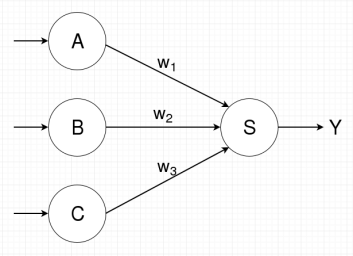
\includegraphics[width=5in]{pic/neuron.png}
\caption{\,\,\,\,\,\,\,\,\,\,Directed graph showing artificial neural network. Source: McGonagle and Belete\cite{McGonagle}}
\label{fig_neuron}
\end{figure}

\subsection{Supervised learning}
This type of machine learning approach basically learns the computer by examples. The algorithm is subjected to a dataset containing features corresponding to labels or targets. For the sake of our earlier example, let's say the labelled dataset are images of handwritten digits annotated to show the corresponding number. With enough training examples, we will train a supervised learning algorithm to recognize the patterns of pixels, edges, corners and shapes related to each digit and ultimately be capable of recognizing handwritten digits and accurately differentiate between digits 3 and 4 or 8 and 0. We can model every supervised learning problem as shown in formula \ref{supervised_formula}.
\begin{equation}
y = f (X),
\label{supervised_formula}
\end{equation}
where $y$ denotes the target classification digit or sometimes called the ground-truth; $X$ denotes the training examples containing \textit{n} number of training examples in the form
\begin{equation}
X = (x_1, x_2,...,x_n),
\end{equation}
$f$ denotes the function the model has to learn from the input data in order to accurately map the input data $X$ to its target output $y$. In this way, the learning model can differentiate its output from the target output in order to discover errors and make adjustments accordingly.

However, supervised learning models need very huge amount of training data in order to generalize very well when fed with unseen data. In this regard, many large datasets have been published and made available to the public. Some examples include Google's Open Images Dataset\footnote{Open Images Dataset - https://research.googleblog.com/2016/09/introducing-open-images-dataset.html} containing about nine million labelled images, Google's labelled video database YouTube-8M\footnote{YouTube-8M - https://research.googleblog.com/2016/09/announcing-youtube-8m-large-and-diverse.html} containing about seven million labelled videos and ImageNet\footnote{ImageNet - http://www.image-net.org/} containing over fourteen categorized images, and many more.

Supervised learning technique can be further grouped into two types. Namely: regression and classification.
\begin{itemize}
    \item\textbf{Linear Regression:} linear regression is used to solve regression problems. Thus it is used for modeling and predicting continuous numeric data. In other words, the aim of linear regression is to construct an algorithm that can take a vector say $x \in \mathbb{R}^n$ as input and predict a scalar value say $y \in  \mathbb{R}$ as output. Let $\hat{y}$ be the predicted value, we define linear regression model in formula \ref{linear_regression_formula}.
    \begin{equation}
        \hat{y} = w^Tx + b,
    \label{linear_regression_formula}
    \end{equation}
    where $w \in \mathbb{R}^n$ is a vector of parameters and $b$ is an intercept term. Some examples of regression applications include predicting stock prices, real-estate prices, weather forecast, etc. Some algorithms of regression include linear regression - the most common algorithm for regression problems, regression tress (ensembles) - sometimes called the decision trees.
    \item\textbf{Classification:} classification is a type of supervised learning technique that is used for simple data - nominal data, categorical data and some numerical variables. Classification can be in two ways: binary and multi-classifications. Binary classification involves classification that produces two possible results, such as Yes/No. Examples include predicting an image as a cat or dog. Multi-classification involves more than two possible outcomes from a given classification problem. For example predicting if a handwritten image is one of any of the nine numbers from zero to nine. 
\end{itemize}
Some popular supervised learning algorithms include: Decision Trees, Linear SVC (Support Vector Classifier), Logistic Regression, Naive Bayes, Neural Networks, Linear Regression, Support Vector Regression (SVR), Gradient boosting and Fisher linear discriminant. 

\begin{figure}[ht]
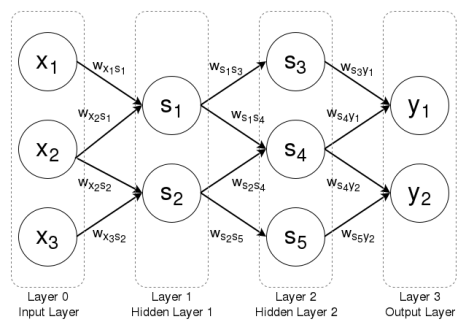
\includegraphics[width=5in]{pic/ANN.png}
\caption{\,\,\,\,\,\,\,\,\,\,A simple ANN consisting of an input layer, two hidden layers and an output layer. Source: McGonagle and Belete\cite{McGonagle}}
\label{fig_ANN}
\end{figure}

\subsection{Unsupervised Learning}
Unsupervised learning is exactly what it sounds. We do not supervise the model but let the model work on its own to discover information from dataset that may not be visible to the human eye. Unsupervised learning uses machine learning algorithms that draw conclusions on unlabeled data. Thus, unsupervised learning studies the way systems can deduce a function to explain the hidden information and structure from unlabelled data. The algorithms in unsupervised learning work to achieve accurate clustering – finding patterns and groupings from unlabeled data. Some popular unsupervised learning algorithms include: K-means clustering, K-NN (K nearest neighbors), Dimensionality Reduction, Neural Networks, Principal Component Analysis, Singular Value Decomposition, Independent Component Analysis, Distribution models and Hierarchical clustering.

Many machine learning technologies can be used to perform both unsupervised learning and supervised learning tasks. For example, the chain rule of probability has it that a vector $x = \mathbb{R}^n$, the joint distribution can be further broken down as shown in formula \ref{eq_unsupervised}.
\begin{equation}
    p(x) = {\displaystyle \prod_{i=1}^{n}}\,p(X_i\,|\,X_1,\dots,X_{i-1}).
    \label{eq_unsupervised}
\end{equation}
From formula \ref{eq_unsupervised}, we can solve the seemingly unsupervised problem of modeling $p(x)$ by dividing it into $n$ supervised learning problems. Instead, we can also solve the supervised problem of learning $p(y\,|\,x)$ by using traditional unsupervised learning methods to learn the joint distribution $p(x,\,y)$, then we infer in formula \ref{eq_unsupervised_further}.
\begin{equation}
    p(y\,|\,x) = \frac{p(x,\,y)}{\sum_y\,p(x,\,y^1)}.
\label{eq_unsupervised_further}
\end{equation}

The biggest difference between supervised and unsupervised learning is that supervised learning deals with labeled data whiles unsupervised learning deals with unlabeled data. Table \ref{diff_supervised_unsupervised} shows the differences between supervised and unsupervised learning.

\begin{center}
\begin{table}
\caption{\,\,\,\,\,Summary of differences between supervised learning and unsupervised learning}
\begin{tabular}{ | m{10em} | m{5cm}| m{5cm} | } 
\hline
\textbf{Criteria} & \textbf{Supervised} & \textbf{Unsupervised} \\ 
\hline
\textbf{Input data} & Uses known labelled data in classes & uses unknown input data  \\ 
\hline
\textbf{Computational Complexity} & More complex in computation MB & Less complex in computation \\ 
\hline
\textbf{Number of classes} & Number of classes is known & Number of classes is not known \\
\hline
\textbf{Real-Time} & Uses offline analysis of data & Uses real-time analysis of data \\
\hline
\textbf{Types} & Two types of supervised machine learning:
\begin{itemize}
    \item Classification
    \item Regression
\end{itemize}& Two types of unsupervised machine learning:
\begin{itemize}
    \item Clustering
    \item Association
\end{itemize}\\
\hline
\end{tabular}
\label{diff_supervised_unsupervised}
\end{table}
\end{center}

\subsection{Semi-supervised Learning}
Semi-supervised learning uses both labelled and unlabelled data. We can say semi-supervised learning lies between supervised and unsupervised learning. In semi-supervised learning, we use some small amount of labelled data to help discover hidden patterns in the rest of the data and improves accuracy. Semi-supervised learning seeks to solve the high cost problem involved in supervised learning. Thus, the cost involved in the process of labelling very large dataset for training is highly reduced in semi-supervised learning. Only few data needs to be labelled to guide a semi-supervised learning model to learn from the rest of the unlabelled data. Semi-supervised approach is very useful in practice as fully labelled data is very difficult and costly to produce compared to unlabelled data. Usually, we use semi-supervised learning when the data acquired needs some special and relevant information or resources in order to be able to achieve training or learning from the data. Some of the methods used in semi-supervised learning include: Generative models, Co-training and multiview models, semi-supervised support vector machines and Graph-based models.

\begin{figure}[ht]
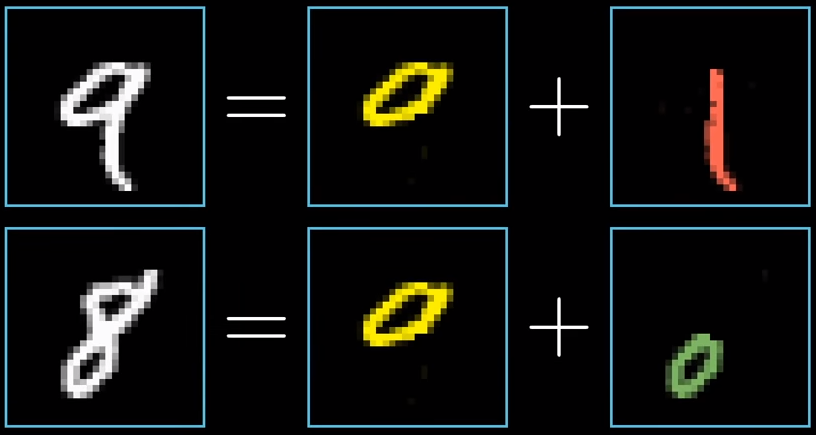
\includegraphics[width=5in]{pic/digits.PNG}
\caption{\,\,\,\,\,\,\,\,\,\,An intuitive breakdown of the digit `8' and `9'. The digit `8' has a loop up top and paired with another loop down low. The digit `9' has a loop up top and a line on the right}
\label{fig_digit}
\end{figure}
\begin{figure}[ht]
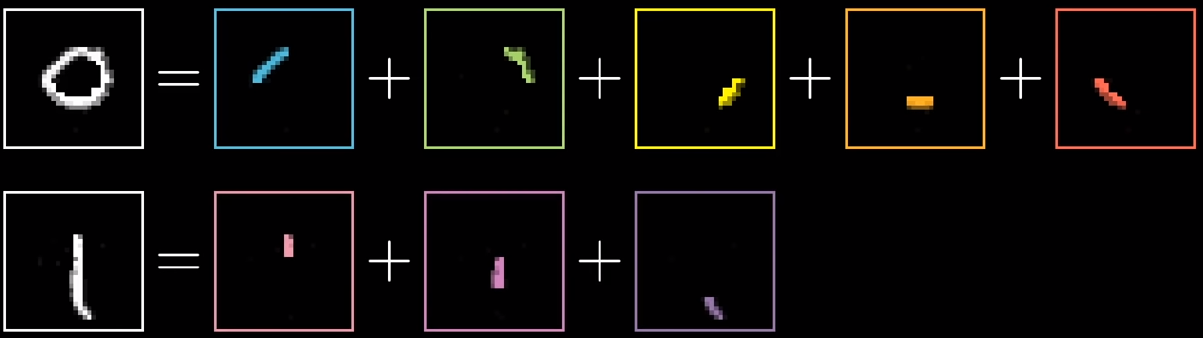
\includegraphics[width=5in]{pic/digits_subcomponents.PNG}
\caption{\,\,\,\,\,\,\,\,\,\,A further breakdown of loops into little edges}
\label{fig_digit_sub}
\end{figure}

Since semi-supervised learning has the same aim of achieving prediction as supervised learning, it can be applied to any problem applicable to supervised learning. For example, semi-supervised learning has been applied in natural language processing (tasks like word sense disambiguation\cite{yarowsky13}, machine translation, sentiment analysis), computer vision, bioinformatics and cognitive psychology.

\section{Deep Learning}
Deep learning is one of the approaches in machine learning that is based on learning the representations in data as compared to other task-specific algorithms. The term deep learning simply means training neural networks or sometimes deep neural networks to learn a general representation of data. The aim of a deep learning network is to estimate some function $f^*$. For instance, for a deep learning classifier, $y = f^*(x)$ tries to map an input $x$ to its corresponding category $y$. A deep learning network defines a mapping $y = f\,(x;\theta)$ and learns the appropriate value of the parameters $\theta$ in order to get the best estimation function. Many deep learning architectures such as \cite{Ivanovsky-2017, Kri12, Chr14}, recurrent neural networks\cite{7914752, 7801769}, and deep belief networks\cite{7111524, 7539822} have been used to solve problems in diverse fields including speech recognition, computer vision, natural language processing, machine translation, etc. However, deep learning can be supervised or unsupervised.

\subsection{Artificial Neural Network}
Artificial Neural networks (ANN) are inspired by the biological neural networks of the animal brain that simply connects many neurons together to form a network. However, in ANN, a neuron is simply a function that takes in input and spits out an output. More formally, we write in formula \ref{ann_formula}. 
\begin{equation}
    z = \vec{w} \cdot \vec{x} + b,
\label{ann_formula}
\end{equation}
where $\vec{w} = (w_1, w_2, \dots, w_n)$ are the weight vectors from previous neurons, $\vec{x} = (x_1, x_2, \dots, x_n)$ are the input units from previous neurons and $b$ is a bias term. Figure \ref{fig_neuron} shows a directed graph of a simple artificial neural network.

Let's go back to our example of recognizing handwritten digits; say our dataset contains grayscale images with size $28 \times 28$ pixels. The network starts with a bunch of neurons corresponding to each of the $28 \times 28$ pixels of the input image which is 784 neurons $(28 \times 28 = 784)$ in total. Each one of these neuron holds a number that represents the grayscale value of the corresponding pixel, ranging from $0$ for black pixels, up to $1$ for white pixels. This number inside the neuron is called its activation. Therefore, all of the 784 neurons form the first layer in the artificial neural network. This artificial neural network will contain a last layer consisting of 10 neurons, with each of the 10 neurons representing one of the digits. The activations (between 1 and 0) in these neurons in the last layer represent how much the network thinks that a given image corresponds with a given digit. There will also be couple layers between the first and last layer called the hidden layers. Figure \ref{fig_ANN} shows a simple artificial neural network with two hidden layers. In a trained ANN, activations in one layer determine activations in the next layer. Meaning, if you feed in an image to the network lighting up all 784 neurons of the input according to the brightness of each pixel in the input image, that pattern of activations causes some specific pattern in the next layer, which causes some pattern in the one after it and so on, which finally gives some pattern in the output layer. In the output layer, the brightest neuron is the network's choice for what digit the input image represents.

In the human eye, when we recognize digits, we piece together various components. The digit `9' has a loop up top and a line on the right as shown in Figure \ref{fig_digit}. The digit `8' also has a loop up top but paired with another loop down low as shown in Figure \ref{fig_digit}. In a perfect artificial neural network, we hope that each neuron from the second to last layer corresponds to one of these sub-components of a handwritten digit. In this way, anytime you feed the network with an image containing a loop up top like `9' or `8', there is some specific neuron whose activation is going to be close to one. In that way, going from the third layer to the last one, it requires learning the appropriate combination of the sub-components that corresponds to which digits. However, recognizing a loop can also be broken down into sub problems. One reasonable way to do this is to first recognize the various little edges that makes it up as shown in Figure \ref{fig_digit_sub}.

Similarly, a long line that you might see in digit one, four or seven is just a long edge or a pattern of several smaller edges. So maybe our hope is that each neuron in the second layer of the network corresponds with the various relevant little edges. We can see that been able to detect edges and patterns like this will be very useful to other image recognition tasks. And even beyond image recognition, there are all sorts of intelligent things we can do that can be broken down into several layers of abstraction. For example speech recognition involves taking raw audios and picking out distinct sounds, which combines to make certain syllabus, which combine to form words, which further combines to make up phrases, and so on.

\begin{figure}[ht]
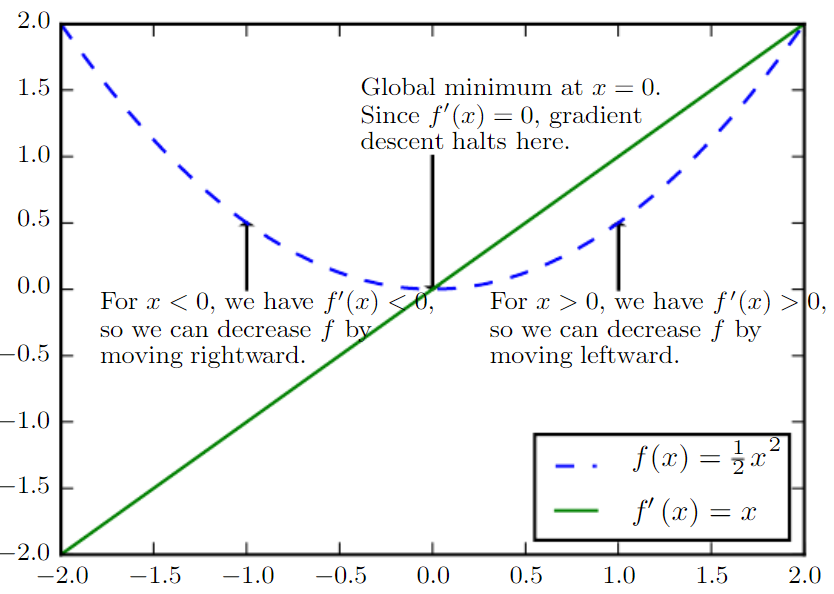
\includegraphics[width=5in]{pic/gradient_descent.PNG}
\caption{\,\,\,\,\,\,\,\,\,\,An illustration of how gradient descent algorithm minimizes the function to the downhill. Source: Goodfellow et al.\cite{Goodfellow-et-al-2016}}
\label{fig_gradient_descent}
\end{figure}

The goal of a neural network in this example is to have some mechanism that can conceivably combine pixels into edges or edges into patterns or patterns into digits. Now to zoom in on one very specific example, let's say the hope of one particular neuron in the second layer of this network shown in Figure \ref{fig_ANN} is to recognize or not if an image has an edge in the middle upper region of the image. The question at hand is what parameters should the network have in order to detect an edge in a said image. To achieve this, we assign a weight to each one of the connections between our neuron and the neurons from the first layer. These weights are just numbers. Then we take all those activations from the first layer and compute their weighted sum according to these weights. We can think about weights as organized in a vector. Let's say green pixels indicate positive weights and the red pixels indicate negative weights with the brightness of the pixel a loose depiction of the weights’ value. If we made the weights associated with almost all of the pixels zero except for some positive weights in the region that we care about; then taking the weighted sum of all the pixel values really just amounts to adding up the values of the pixel in just the region we care about. When we compute the weighted sum we might come up with any number; but for artificial neural network what we want is for activations to be some value between zero and one. So the common thing to do is to push this weighted sum into some function that squashes the number into the range that is between zero and one. There are many functions that do this. Some these functions include: Sigmoid, Tanh, Rectified linear unit (ReLU), Leaky rectified linear unit (Leaky ReLU), Parametric rectified linear unit (PReLU), Exponential linear unit (ELU), etc. At this stage, we can rewrite our neuron formula with the activation function $H$ as outlined in formula \ref{equation_vec}.
\begin{equation}
    H(\vec{w} \cdot \vec{x} + b)
\label{equation_vec}
\end{equation}
Hence, activation of the neuron is basically a measure of how positive the relevant weighted sum is. But maybe we don't want a neuron to light up when the weighted sum is bigger than zero. Maybe we only want a neuron to be active when the weighted sum is bigger than say 10. That is, we want some bias for it to be active. What we can do is to add some number say $-10$ to the weighted sum before plugging into the squashing function. That additional number is called the bias term, $b$. Therefore, the weights tells us what pixel pattern the neuron in the second layer is picking up on and the bias tells us how high the weighted sum needs to be before the neurons start getting meaningfully active. And this whole process is for just one neuron. Every other neuron in the second layer is going to be connected to all $784$ neurons from the first layer. And each of the $784$ connections has its own weight associated with it. Also, each one has some bias. So if this hidden layer has $16$ neurons, that's a total of $784 \times 16$ weights along $16$ biases. All of that are just the connections from the first layer to the second. The connections between the other layers also have a bunch of weights and biases associated with them. All said and done, this network has bunch of weights and biases that can tweaked and turned to make this network behave in different ways. In essence, learning or training an ANN is getting the network to find the right weights and biases so that it can actually make accurate classification from given data. It is obviously impractical to set all these weights and biases by hand.

We write down the equation of an artificial neural network in a more compact notational way in equation \ref{ANN_equation}, we can organize all activations from one layer into a column as a vector. We can also organize all the weights as a matrix, where each row of the matrix corresponds to the connections between one layer and a particular neuron in the next layer. Thus, taking the weighted sum of the activations in the first layer corresponds to one of the terms in the matrix vector product. Furthermore, instead of adding the bias to each of these values independently, we represent it by organizing all those biases into a vector and adding the vector to the previous matrix vector product. Then in the final step, we wrap a squashing function around the entire expression. What that's supposed to represent is that we will apply the squashing function to each specific component of the resulting vector inside. In summary, the entire network is just a function that takes in 784 numbers as an input and spits out 10 numbers as an output. It is absurdly complicated function that involves so many parameters in the form of weights and biases that pick up on certain patterns, and which involves iterating many matrix vector products and a squashing function.
\begin{equation}
    a^1 = 
H\begin{pmatrix}\begin{bmatrix}
  w_{0,0} & w_{0,1} & \cdots & w_{0,n} \\
  w_{1,0} & a_{2,2} & \cdots & w_{1,n} \\
  \vdots  & \vdots  & \ddots & \vdots  \\
  w_{m,0} & w_{m,1} & \cdots & w_{m,n} 
 \end{bmatrix}
 \begin{bmatrix}
  a_0^{(0)} \\
  a_1^{(0)} \\
  \vdots \\
  a_n^{(0)} 
 \end{bmatrix} + 
 \begin{bmatrix}
  b_0 \\
  b_1 \\
  \vdots \\
  b_n 
 \end{bmatrix}\end{pmatrix}
 \label{ANN_equation}
\end{equation}

\subsection{Cost function - how neural networks get punished}
Conceptually, we think of each neuron as been connected to all of the neurons in the previous layer, with the weights and weighted sum defining its activation whiles the bias is some indication of whether the neuron is active or inactive. In artificial neural network, we will start by initializing all the weights and biases totally randomly. That is, the network is going to perform pretty bad on some given examples since it is just doing something random. For example, if we feed in an input image of a $3$, the output layer gets confused and utters out trash. So what we will do is to define a cost function $E_{total}$, a way of telling the computer that the output should have activations which are $0$ for most neurons but $1$ for the image class neuron. In a mathematical language, we'll add up the squares of the differences between each of those trash output activations and the value that we want them to have as shown in equation \ref{cost_function}.
\begin{equation}
    E_{total} = \frac{1}{n}\sum_{i=1}^{n} (Y_i - \hat{Y}_i)^2
    \label{cost_function}
\end{equation}

\begin{figure}[ht]
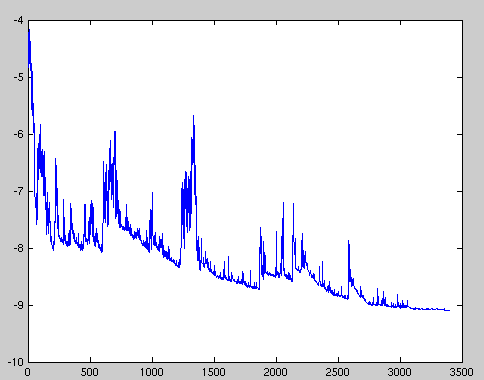
\includegraphics[width=5in]{pic/fluctuation.png}
\caption{\,\,\,\,\,\,\,\,\,\,Objective function fluctuations caused by high variance of frequent updates}
\label{SGD}
\end{figure}

In this sense, the sum, $E_{total}$ is small when the network confidently classifies the image correctly but it is large when the network seems like it does not really know what it is doing. Furthermore, we consider the average cost over all the dataset samples at our disposal. This average cost is our measure of how good or bad the network is performing. The ANN itself is basically a function; taking in 748 pixels as input and outputs 10 numbers and parameterized by so many weights and biases. Here, the cost function is a layer of complexity on top of that. It takes as input those many weights and biases and outputs a single number describing how bad or good those weights and biases are; and its defined based on the network's behaviour over all the tens of thousands of pieces of training data. There are many forms of cost functions such as Cross-entropy cost\cite{deBoer2005} for multi-class classification, Hellinger distance\cite{Nikulin2018}, Kullback–Leibler divergence\cite{kullback1951}, Generalized Kullback–Leibler divergence\cite{4655451}, Itakura–Saito distance\cite{NOZAKI201763}, etc.

\subsection{Gradient Descent - how neural networks are corrected}
Telling the computer what kind of a bad job it is doing is not really helpful. We want to tell it how to change those weights and biases so that it gets better. At this point let us imagine we have a simple function, which has one number as an input and one number as an output. Our job is to find an input that minimizes the value of this function. In calculus, you can sometimes figure out this minimum number explicitly; but not always feasible for a very complicated function. Certainly not feasible in our very complicated neural network cost function. 

\begin{figure}[ht]
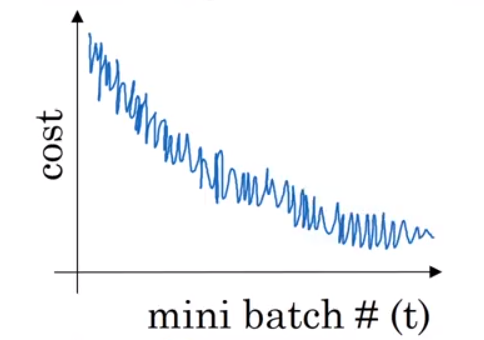
\includegraphics[width=5in]{pic/mini-batch.PNG}
\caption{\,\,\,\,\,\,\,\,\,\,Mini-batch gradient descent variance of objective function (cost function). There is little bit of fluctuations due to some difficult mini-batch examples.}
\label{mini-batch}
\end{figure}

A more flexible tactic is to start out at any input and figure out which direction we should step to make that output lower. Specifically, if we can find out the slope of the function where we are then shift to the left if that slope is positive and shift to the right if the slope is negative. If we do this repeatedly, at each point checking the new slope and taking the appropriate step, we are going to approach some local minimum of the function. An image we might have in mind here is a ball rolling down a hill. We must mention that even for this really simplified input function, there are many possible values that you might land in depending on which random input you start at. Hence, there is no guarantee that the local minimum you land in is going to be the smallest possible value of the cost function. Furthermore, if we make our step sizes proportional to the slope, then when the slope is flattening out towards the minimum, our steps gets smaller and smaller. And this will help us from over shooting.
Imaging a function instead of two inputs and one output; we might think of the input space as a $xy$ plane; and the cost function as been graphed as a surface above it. Instead of finding the slope of the function, we will find the direction to step in this input space so as to decrease the output of the function most quickly. In other words what is the downhill direction? And again, it is helpful to think of a ball rolling down that hill. In multi-variable calculus, the gradient of a function gives us the direction of steepest ascent. Basically, which direction should you step to increase the function most quickly. Naturally, taking the negative of that gradient gives you the direction to step that decreases the function most quickly. And even more than that, the length of this gradient vector is actually an indication for just how steep that steepest slope is. In summary, the algorithm for minimizing the function is to compute this gradient direction, then take a small step downhill and repeat that over and over.
Figure \ref{fig_gradient_descent} shows a demonstration of the gradient descent. We summarize gradient descent algorithm as follows:
We begin with iteration as $i = 0$ and a starting position on the hill, $x_i$.
\begin{algorithm}[H]
\SetAlgoLined
\KwResult{$x_i$ minimum }
 \While{$i < epochs$}{
  
  \eIf{$x_i \neq MINIMUM$}{
   $p_i$,  compute vector distance in $n-$space
   
   $\alpha_i \ni f(x_i + \alpha_ip_i) < f(x_i)$,  compute the step length
   
   $i = i + 1$,  update the variables
   }{
   RETURN $x_i$\;
  }
 }
 \caption{Algorithm for gradient descent}
\end{algorithm}

Therefore, with our cost function, changing the weights and biases to decrease the cost function value means making the output of the network on each piece of training data look less of a random array of ten values and more like an actual decision that we wanted to make. It is important to remember that this cost function involves an average over all of the training data. Consequently, minimizing the cost function means our network performs better on all of those training samples. In essence, what it means for a neural network to learn is all about minimizing the cost function.

Gradient Descent is one of the most popular ways to train and optimize a neural network. There are mainly three forms of gradient descent algorithm with difference in how much data is used to update the gradient of the relating function.

\begin{figure}[ht]
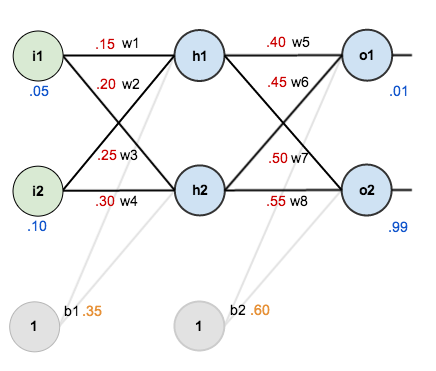
\includegraphics[width=5in]{pic/network_example2.png}
\caption{\,\,\,\,\,\,\,\,\,\,Structure of a neural network with two input $i_1, i_2$,  two hidden neurons $h_1, h_2$, two output neurons $o_1, o_2$, two biases $b_1, b_2$ and eight weights $w_1, \cdots, w_8$.}
\label{neural_net_example}
\end{figure}

\subsubsection{Batch gradient descent}
Batch gradient descent is a form of gradient descent algorithm that calculates the gradient of the cost function with respect to the the parameters $\theta$ for the entire training dataset. Mathematically, we show in equation \ref{bgd_formula}.
\begin{equation}
    \theta = \theta - \eta \cdot \nabla_\theta J(\theta)
\label{bgd_formula}
\end{equation}
where $\eta$ is the learning rate that determines how big to update the parameters $\theta$, and $\nabla_\theta J(\theta)$ is the differentiation of gradients with respect to some parameters $\theta$. Batch gradient descent need all training examples in order to perform parameter updates. Hence, the algorithm becomes very slow and difficult to deal with dataset that can't fit into memory at once. Furthermore, batch gradient descent is not suitable for training online models as new dataset examples can't be fed to the model once we begin training. 

\subsubsection{Stochastic gradient descent}
Unlike batch gradient descent, stochastic gradient descent updates the parameters for every training example $x^{(i)}$ and label $y^{i}$. Mathematically, we show in equation \ref{sgd_formula}.
\begin{equation}
    \theta = \theta - \eta \cdot\nabla_\theta J(\theta;x^{(i)};y^{(i)}).
\label{sgd_formula}
\end{equation}
Stochastic gradient descent (SGD) solves the problems of slow training and online training in batch gradient descent. As each dataset example is fed to the model at a time, we can compute the gradient faster and update the parameters at a time. The algorithm is also suitable for online model training, we feed new dataset examples to the model as and when they arrive. However, with the frequent update performed on every single dataset example, SGD has high variance in updates and causes fluctuations in the objective function as shown in Figure \ref{SGD}.

\begin{figure}[ht]
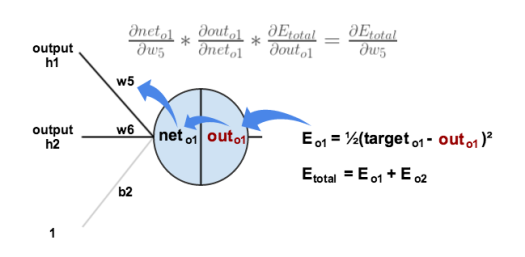
\includegraphics[width=5in]{pic/output_1_backprop-4.png}
\caption{\,\,\,\,\,\,\,\,\,\,Back propagation of the error for $o_1$ and $o_2$}
\label{output_1_backprop}
\end{figure}

\begin{figure}[ht]
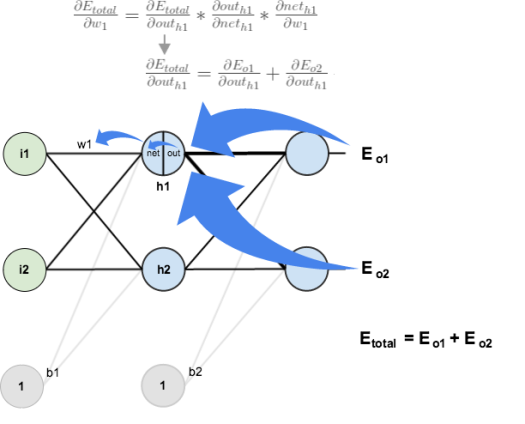
\includegraphics[width=5in]{pic/nn-calculation.png}
\caption{\,\,\,\,\,\,\,\,\,\,Back propagation the error of $o_1$ and $o_2$ to obtain $w_{2}^{\prime}, w_{3}^{\prime}$ and $w_{4}^{\prime}$ for $w_2, w_3$ and $w_4$ respectively}
\label{fig_nn-calculation}
\end{figure}

\subsubsection{Mini-batch gradient descent}
Mini-batch gradient descent combines the advantages of batch gradient descent and SGD and performs parameter updates for every mini-batch of $n$ training examples. Mathematically, we show in equation \ref{mbgd_formula}.
\begin{equation}
    \theta = \theta - \eta \cdot \nabla_\theta J(\theta; x^{(i:i+n)}; y^{(i:i+n)}).
\label{mbgd_formula}
\end{equation}
For mini-batch gradient descent, the cost function is calculated over some small number of training examples (usually between 10 - 500). This is in contrast with batch gradient descent of the entire training examples and SGD of one training example. Also, mini-batch gradient descent do not cause fluctuations in the objective function as update is done over reasonable amount of training examples as shown in Figure \ref{mini-batch}.

\subsection{Back propagation - how neural networks learn}
Back propagation is the core algorithm behind how neural networks learn. Back propagation is an algorithm for minimizing the cost function. Because the cost function involves averaging a certain cost per example over all the tens of thousands of training examples, the way that we adjust the weights and biases for a single gradient descent step also depends on every single example. Let's take for example feeding an image of digit \textit{2}  into an artificial neural network that is not trained yet. Since the network is not trained yet, the activations in the output layer are going to be pretty random. Here, we cannot directly change the activations in the output layer; instead we can only change the weights and biases of the network. But it is helpful to keep track of which adjustments we wish to take place to that output layer. And since we want it to classify the image as a digit \textit{2} , we will want say the value in the third output layer neuron be nudged up whiles all of the others get nudged down. Moreover, the sizes of these nudges should be proportional to how far away each current value is from its target value. For example, the increase to the number two's neuron activation is in essence more important than the decrease in the number eight's neuron. Let's zoom in further and focus on just the digit \textit{2} neuron. We already know that activations are made up of the weighted sum of all the activations in the previous layer plus a bias which is all then plugged into some squash function as stated in equation \ref{ANN_equation}. Hence, there are three different avenues that team up together to help increase that activation; we can increase the bias, we can increase the weight, and we can change the activations of the previous layers.

Focusing on how the weights should be adjusted, the weights actually have different levels of influence. The connection with the brightest neurons from the preceding layer, have the biggest effect since those weights are multiplied by larger activation values. So if we increase those weights, it actually has a strong influence on the ultimate cost function than increasing the weights of connections with dimmer neurons as far as this training example is concern. Remember, when we talked about gradient descent, we don't just care about whether each component should get nudged up or down. We care about which components have the most effect on cost function. This by the way is at least going to get someone reminiscing of the theory in neural science for how biological neurons learn, called Hebbian theory\cite{Donald1949}. This theory is often summed up in the phrase ``Neurons that fire together wire together''. Here, the biggest strengthening of connections happens between neurons which are the most active and the ones which we wish to become more active. In essence, the neurons which are firing whiles seeing a digit \textit{2} gives more strongly linked to those firing whiles thinking about a digit \textit{2}. To be clear, really we are not in a position to be making statements one way or another about whether artificial networks of neurons behaves any a thing like biological brains. But taking as a very loose analogy, we do find it interesting to note.

\begin{figure}[ht]
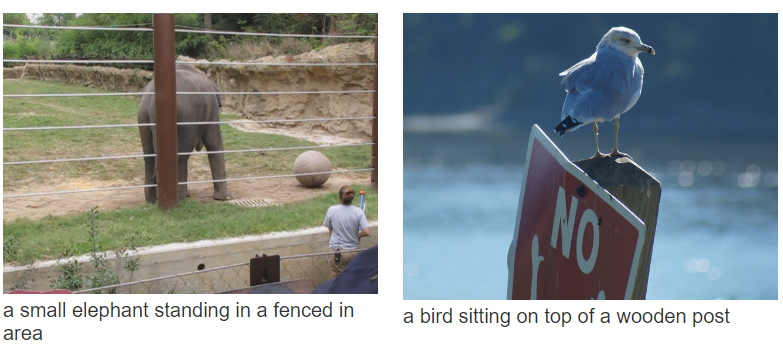
\includegraphics[width=5in]{pic/CNN_example.PNG}
\caption{\,\,\,\,\,\,\,\,\,\,ConvNet recognizing scenes and accurately suggesting important captions. Source: Johnson et al.\cite{densecap}}
\label{cnn_example}
\end{figure}

\begin{figure}[ht]
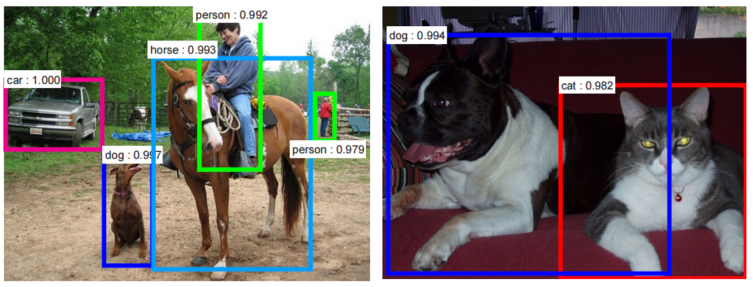
\includegraphics[width=5in]{pic/everyday_objects.PNG}
\caption{\,\,\,\,\,\,\,\,\,\,ConvNet recognizing everyday objects with bounding boxes. Source: Ren et al.\cite{DBLP:journals/corr/RenHG015}}
\label{everyday_objects}
\end{figure}

\begin{figure}[ht]
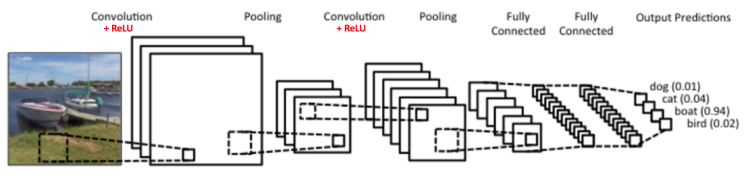
\includegraphics[width=5in]{pic/ConvNet_Arch.png}
\caption{\,\,\,\,\,\,\,\,\,\,A simple ConvNet architecture. Source: Ujjwalkarn\cite{intuitiveCNN}}
\label{ConvNet_arch}
\end{figure}

The third way is that we can help increasing the activation of the output neuron corresponding to the digit \textit{2} is by changing all the activations in the previous layer. Namely, if everything connected to that digit \textit{2} neuron with a positive weight got brighter; and everything connected with a negative weight got dimmer; then that digit \textit{2} neuron will become more active. Similar to the weight changes, there is stronger effect by seeking changes that are proportional to the size of the corresponding weights. Of course, we cannot directly influence those activations, we only have control over the weights and biases. Let us keep in mind that what we actually want is the output layer to have all other neurons be less active except the digit two neuron to be highly active. However, each of those output neurons have their own thoughts about what should happen to that second to last layer. Hence, the desire of the digit two neuron is added together to the desires of all the other output neurons for what should happen to this second to last layer; this should be done in proportion to the corresponding weights and in proportion to how much each of those neurons needs to change.

This is where the idea of propagating backwards comes in. When adding together all these desired effects, we basically give a list of nudges that we want to happen to the second to last layer. And once we have those, we can recursively apply the same process to the relevant weights and biases that determines those values, repeating the same process that we just walked through and moving backwards through the network. Zooming out a bit further, this is all what a single training step wishes to nudge each one of those weights and biases. If we only feed the network with a digit \textit{2} image, the network will ultimately be incentivized to classify all images as a \textit{2}. So what we do is to go through this same back propagation routine for every other training example recording how each of them will like to change the weights and the biases; then we average together those changes. This collection here of the average nudges to each weights and biases is loosely speaking the negative gradient of the cost function or something proportional to it. In practice it takes computers a very long time to add up the influence of every single training example and every single gradient descent step. So here is what is commonly done instead, we randomly shuffle the training data and divided it into a whole bunch of mini-batches. Say each batch containing a hundred training examples. Then we compute the gradient descent step using back propagation according to the mini-batch. That is not going to be the actual gradient of the cost function because it does not depend on all the training data but a single subset and not the most efficient step downhill. But each mini-batch does give a pretty good approximation and more importantly gives a significant computational speed up. If you plot the trajectory of the network under the relevant cost surface, it will be more like a drunk man stumbling in a slay down a hill but taking quick steps rather than a carefully calculated man taking the exact downhill direction of each step before taking a very slow and careful step in that direction.

In summary, back propagation is the algorithm for determining how a single training step would like to update the weights and biases; not only in terms of whether the weights and biases should go up or down but also in terms of what relative proportions to those changes causes the most rapid decrease to the cost. A true gradient descent step will involve repeating a back propagation for all the tens and thousands of training examples and averaging the desired changes. But that is computationally slow, so instead we randomly sub divide the data into mini-batches and compute each step with respect to a mini-batch. Repeatedly going through all of the mini-batches, and making the weights and biases adjustments, we will converge towards a local minimum of the cost function. Thus, the network will end up doing a really good job on the training examples.

\begin{figure}[ht]
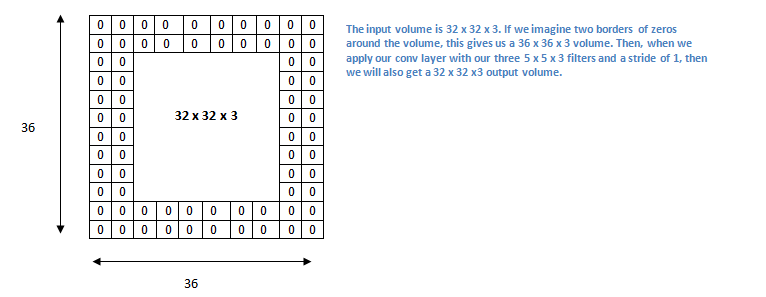
\includegraphics[width=7in]{pic/padding.png}
\caption{\,\,\,\,\,\,\,\,\,\,Padding a 32$\times$32$\times$3 input image into a 36$\times$36$\times$3}
\label{fig_padding}
\end{figure}

\begin{figure}[ht]
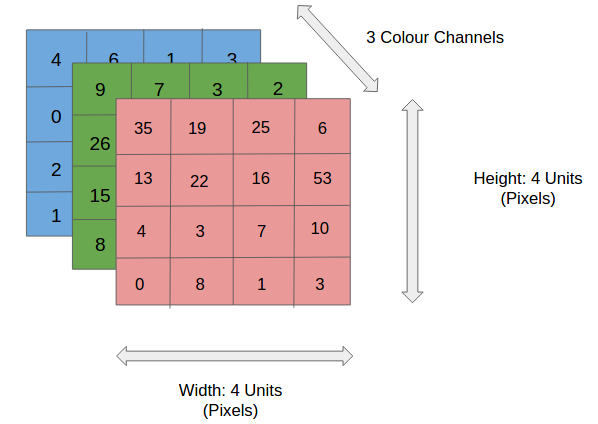
\includegraphics[width=5in]{pic/rgb_image.png}
\caption{\,\,\,\,\,\,\,\,\,\,An RGB image with volume of size: 4 x 4 x 3. It comprises of the 3 Colour channel matrices: Source \cite{Abhineet}}
\label{rgb_image}
\end{figure}

\section{Putting all together}
We will consider a neural network with two inputs $i_1, i_2$, two hidden neurons $h_1, h_2$ and two output neurons $o_1, o_2$. Also, we apply bias $b_1, b_2$ to the hidden and output neurons respectively. The neural network has eight weights $w_1, \cdots, w_8$ as shown in Figure \ref{neural_net_example}. We randomly initialize the inputs/outputs, weights and biases. The aim of the network is to output $0.01$ and $0.99$ corresponding to some given arbitrary input $0.05$ and $0.10$.
We begin training by forward pass with the randomly initialized parameters. We compute the net input for $h_1$ and $h_2$ as follows:\\
\textbf{Compute weights} \\
To compute net input for $h_1$, we have:
\[net_{h1} = w_1 * i_1 + w_2 * i_2 + b_1 * 1\]
\[net_{h1} = 0.15 * 0.05 + 0.2 * 0.1 + 0.35 * 1 = 0.3775\]
we use logistic function for activation:
\[output_{h1} = \frac{1}{1 + e^{-net_{h1}}} = \frac{1}{1 + e^{0.3775}} = 0.593269992\]
we perform same process to compute net input for $h_2$:
\[output_{h2} = 0.596884378\]
To compute $o_1$ and $o_2$, we go through same process\\
for $o_1$:
\[net_{o_1} = w_5 * output_{h_1} + w_6 * output_{h_2} + b_2 * 1\]
\[net_{o_1} = 0.4 * 0.59326992 + 0.45 * 0.596884378 + 0.61 * 1 = 1.105905967\]
\[output_{o_1} = \frac{1}{1 + e^{-net_{o_1}}} = \frac{1}{1 + e^{-1.105905967}} = 0.75136507\]
repeating same process for $o_2$, we have:
\[output_{o_2} = 0.772928465 \]
\textbf{Compute error} \\
We calculate the network error using the mean squared error function, given in equation \ref{cost_function}\\
For $o_1$ with predicted output, $\hat{Y}$ as $0.75136507$ and target $Y$ as 0.01, we compute the error as follows:
\[E_{o_1} = \frac{1}{n}(Y_{o_1} - \hat{Y}_{o_1})^2 = \frac{1}{2}(0.01 - 0.75136507)^2 = 0.274811083\]
applying same process for $o_2$ with predicted output, $\hat{Y}$ as $0.772928465$ and target $Y$ as 0.99, we have:
\[E_{o_2} = 0.023560026\]
we compute total network error as:
\[E_{total} = E_{o_1} + E_{0_2} = 0.274811083 + 0.023560026 = 0.298371109\]
\textbf{Back propagation} \\
We take the weight $w_5$ and compute how much effect it has on the total error, we apply the chain rule to get:
\[\frac{\partial E_{total}}{\partial w_5} = \frac{\partial E_{total}}{\partial output_{o_1}} * \frac{\partial output_{o_1}}{\partial net_{o_1}} * \frac{\partial net_{o_1}}{\partial w_5}\]
we can visualize this operation in Figure \ref{output_1_backprop}. We compute the effect of the total error $E_{total}$ w.r.t. the outputs $o_1$ and $o_2$.
\[ E_{total} = \frac{1}{2}(Y_{o_1} - \hat{Y}_{o_1})^2 + \frac{1}{2}(Y_{o_2} - \hat{Y}_{o_2})^2 \]
\[ \frac{\partial E_{total}}{\partial output_{o_1}} = 2 * \frac{1}{2}(Y_{o_1} - \hat{Y}_{o_1})^{2-1} * -1 + 0 \]
\[ \frac{\partial E_{total}}{\partial output_{o_1}} = -(Y_{o_1} - \hat{Y}_{o_1}) = (0.01 - 0.7513607) = 0.74136507 \]
Next, we compute how much the the output $o_1$ changes w.r.t. its corresponding total net input
\[ \frac{\partial output_{o_1}}{\partial net_{o_1}} = output_{o_1}(1 - output_{o_1}) = 0.75136507(1 - 75136507) = 0.186815602 \]
Finally, we compute how much change of the total net input of output $o_1$ w.r.t. $w_5$
\[ net_{o_1} = (w_5 * output_{h_1}) + (w_6 * output_{h_2}) + (b_2 * 1) \]
\[ \frac{\partial net_{o_1}}{\partial w_5} = 1 * output_{h_1} * w^{(1-1)}_{5} + 0 + 0 = output_{h_1} = 0.593269992 \]
Therefore, 
\[ \frac{\partial E_{total}}{\partial w_5} = \frac{\partial E_{total}}{\partial output_{o_1}} * \frac{\partial output_{o_1}}{\partial net_{o_1}} * \frac{\partial net_{o_1}}{\partial w_5}\]
\[ \frac{\partial E_{total}}{\partial w_5} = 0.74136507 * 0.186815602 * 0.593269992 = 0.082167041 \]
We decrease the error by subtracting this value $\frac{\partial E_{total}}{\partial w_5}$ from the current weight value $w_5$ and multiplied by a learning rate $\eta$.
\[ w^{\prime}_{5} = w_5 - \eta * \frac{\partial E_{total}}{\partial w_5} = 0.4 - 0.5 * 0.082167041 = 0.35891648 \]
we compute new weights for $w_6, w_7, w_8$ following the same process to obtain
\[ w^{\prime}_{6} = 0.408666186 \]
\[ w^{\prime}_{7} = 0.511301270 \]
\[ w^{\prime}_{8} = 0.561370121 \]
\textbf{Hidden layer}\\
Next, we continue the back prop in a similar process for the outputs layer neurons $o_1$ and $o_2$ to update weights $w_1, w_2, w_3,$ and $w_4$ of the hidden layer using the equation below
\[ \frac{\partial E_{total}}{\partial w_1} = \frac{\partial E_{total}}{\partial output_{h_1}} * \frac{\partial output_{h_1}}{\partial net_{h_1}} * \frac{\partial net_{h_1}}{\partial w_1} \]
but we know 
\[ \frac{\partial E_{total}}{\partial output_{h_1}} = \frac{\partial E_{o_1}}{\partial output_{h_1}} + \frac{\partial E_{o_2}}{\partial output_{h_1}} \]
for $\frac{\partial E_{o_1}}{\partial output_{h_1}}$, we have 
\[ \frac{\partial E_{o_1}}{\partial output_{h_1}} = \frac{\partial E_{o_1}}{\partial net_{h_1}} * \frac{\partial net_{o_1}}{\partial output_{h_1}} \]
we compute $\frac{\partial E_{o_1}}{\partial net_{o_1}}$ from our already obtained values as
\[ \frac{\partial E_{o_1}}{\partial net_{o_1}} = \frac{\partial E_{o_1}}{\partial output_{o_1}} * \frac{\partial output_{o_1}}{\partial net_{o_1}} = 0.74136507 * 0.186815602 = 0.138498562\]
also, $\frac{\partial net_{o_1}}{\partial output_{h_1}}$ is equal to $w_5$
\[ net_{o_1} = w_5 * output_{h_1} + w_6 * output_{h_2} + b_2 * 1 \]
\[ \frac{\partial net_{o_1}}{\partial output_{h_1}} = w_5 = 0.40 \]
we put our obtained values into
\[ \frac{\partial E_{o_1}}{\partial output_{h_1}} = \frac{\partial E_{o_1}}{\partial net_{o_1}} * \frac{\partial net_{o_1}}{\partial output_{h_1}} = 0.138498562 * 0.40 = 0.055399425 \]
we follow same process to compute $\frac{\partial E_{o_2}}{\partial output_{h_2}}$
\[ \frac{\partial E_{o_2}}{\partial output_{h_2}} = -0.019049119 \]
Hence, we have
\[ \frac{\partial E_{total}}{\partial output_{h_1}} = \frac{\partial E_{o_1}}{\partial output_{h_1}} + \frac{\partial E_{o_2}}{\partial output_{h_1}} = 0.055399425 + -0.019049119 = 0.036350306\]
So far, we have obtained $\frac{\partial E_{total}}{\partial h_1}$, we need to calculated $\frac{\partial output{h_1l}}{\partial h_1}$ and $\frac{\partial net_{h_1}}{\partial w}$ for each weight:
\[ output_{h_1} = \frac{1}{1 + e^{-net_{h_1}}} \]
\[ \frac{\partial output_{h_1}}{\partial net_{h_1}} = output_{h_1}(1 - output_{h_1}) = 0.5932699(1 - 0.59326999) = 0.241300709  \]
we compute the $\frac{\partial net_{h_1}}{\partial w_2}$ same way as the output neurons $o_1$ and $o_2$
\[ net_{h_1} = (w_1 * i_1) + (w_3 * i_2) + (b_1 * 1) \]
\[ \frac{\partial net_{h_1}}{\partial w_1} = i_1 = 0.05 \]
now we plug in all values obtained into
\[ \frac{\partial E_{total}}{\partial w_1} = \frac{\partial E_{total}}{\partial output_{h_1}} * \frac{\partial output_{h_1}}{\partial net_{h_1}} * \frac{\partial net_{h_1}}{\partial w_1} \]
\[ \frac{\partial E_{total}}{\partial w_1} = 0.036350306 * 0.241300709 * 0.05 = 0.000438568 \]
at this point, we can compute and update $w_1$ as
\[ w_{1}^{\prime} = w_1 - \eta * \frac{\partial E_{total}}{\partial w_1} = 0.15 - 0.5 * 0.000438568 = 0.149780716 \]
we repeat same process to obtain $w_{2}^{\prime}, w_{3}^{\prime}$ and $w_{4}^{\prime}$ for $w_2, w_3$ and $w_4$ respectively. Figure \ref{fig_nn-calculation} shows a visualization of this process.
\[ w_{2}^{\prime} = 0.19956143 \]
\[ w_{3}^{\prime} = 0.24975114 \]
\[ w_{4}^{\prime} = 0.29950229 \]

Eventually, we have updated all the weights in our neural network. Initially, the network error was 0.298371109 for inputs 0.05 and 0.1. After the first epoch we reduce the network error to 0.291027924. We didn't achieve much error reduction after the first epoch, but after iterating this procedure 10,000 times, we reduce the network error drastically to 0.0000351085. At this moment, when we feed our network with the input 0.05 and 0.1, the network outputs 0.015912196 for the 0.01 ground-truth and 0.984065734 for 0.99 ground-truth.

\section{Convolutional Neural Networks}
A Convolutional Neural Network (CNN or ConvNets) is a type of artificial neural network that uses filters or kernels to perform convolution on inputs to extract useful information. In recent years, ConvNets have been very successful in solving computer vision problems such as image recognition and classification. Apart from empowering the vision of robots and self driving cars, ConvNets have been very effective in recognizing faces, detecting objects, etc. Figure \ref{cnn_example} shows ConvNet recognizing scenes and accurately suggesting important captions ("a small elephant standing in a fenced in area"). In Figure \ref{everyday_objects}, ConvNet is used to recognize objects that appear in everyday life with very high accuracy. Therefore, ConvNets are relevant tool to use in many machine learning problems, especially in the field of computer vision. A ConvNet normally include number of convolutional layer plus non linearity (ReLU) and pooling layers that may be followed by some fully connected layers. These processes are the main building blocks of every ConvNet architecture. Figure \ref{ConvNet_arch} depicts a ConvNet architecture that learns to classify images into four categories: dog, cat, boat or bird. A ConvNet normally takes as input an order 3 tensor, thus, an input image with \textit{H} rows, \textit{W} columns, and 3 channels (R, G, B image color channels). The input image is then passed through series of processes (convolution, ReLU, fully connected layers). We can abstract the whole ConvNet structure as illustrated in equation \ref{ConvNet_structure}.
\begin{equation}
x^1 \rightarrow \boxed{ w^1 } \rightarrow  x^2 \rightarrow ... \rightarrow  x^{L-1} \rightarrow \boxed{ w^{L-1} } \rightarrow  x^L  \rightarrow \boxed{ w^L }  \rightarrow z
\label{ConvNet_structure}
\end{equation}
In equation \ref{ConvNet_structure}, we show how ConvNet process input image in a forward pass.

\begin{figure}[ht]
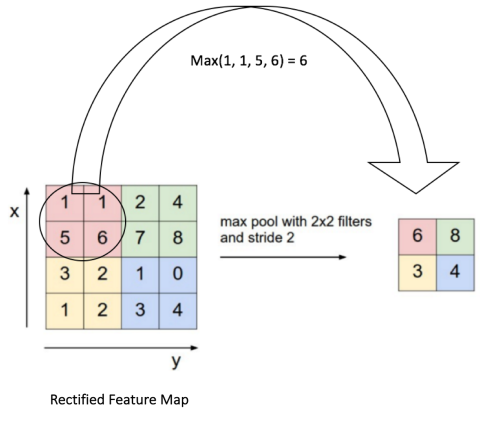
\includegraphics[width=5in]{pic/pooling.png}
\caption{\,\,\,\,\,\,\,\,\,\,Max Pooling. We slide a $2 \times 2$ window by 2 strides over a $4 \times 4$ rectified feature map and take the maximum value in each region to obtain a $2 \times 2$ output.}
\label{fig_maxpooling}
\end{figure}

\subsection{Convolution layer}
Actually, we can represent every image as a matrix containing pixel values. A standard color image contains three channels - red, green and blue, commonly refered to as RGB. Each of these three channels is a 2d-matrice stacked on top of each other with each containing pixel values ranging from 0 to 255 as shown in Figure \ref{rgb_image}. On the other hand, a grayscale image contains only one channel, thus, just one 2d-matrix having pixel values from 0 to 255 with pixel values close to 0 representing black color and pixel values close to 255 representing white color. A convolution operation is an element-wise dot product multiplication of two matrices. Let us take for example convolution of a 5 x 5 matrix and a 3 x 3 matrix as shown in Figure \ref{fig:convolution}. Consequently, the convolution computation of the $5 \times $5 matrix and the $3 \times $3 matrix is shown in equation \ref{conv_operation}.

\begin{equation}
\begin{bmatrix}
1 & 1 & 1 & 0 & 0 \\
0 & 1 & 1 & 1 & 0 \\
0 & 0 & 1 & 1 & 1 \\
0 & 0 & 1 & 1 & 0 \\
0 & 1 & 1 & 0 & 0
\end{bmatrix}
\cdot
\begin{bmatrix}
1 & 0 & 1 \\
0 & 1 & 0 \\
1 & 0 & 1
\end{bmatrix}
=
\begin{bmatrix}
4 & 3 & 4 \\
2 & 4 & 3 \\
2 & 3 & 4
\end{bmatrix}
\label{conv_operation}
\end{equation}

For a typical convolutional layer, it is made up of set of filters that will be learned during training. Every filter is actually a small matrix with equal channel size as the input image depth. For example, an RGB input image of size 128 x 128 x 3 will have corresponding filters of size 5 x 5 x 3 (thus, a square matrix with 5 pixels width and height and 3 channels to correspond to the input image 3 color channels). During feed forward pass, every filter slide or convolve spatially over the entire input image and compute dot products of the corresponding entries of the filter and the input image. The output of the convolve operation is a 2-dimensional feature map or activation map. We expect the convnet to learn appropriate filters that will activate for some type of visual features such as edges, shapes, and even objects.   

After performing convolution computation on an image, the spatial size of the output may shrink and information contained in that part will be lost. To solve this problem, we use padding. Padding is simply wrapping around the input image with additional lines (usually with zeros or some other values). Figure \ref{fig_padding} shows padding of an input image of size 32$\times$32$\times$3 with zeros, the image size now becomes 36$\times$36$\times$3. Performing convolution operation on the new image with a filter of size 5$\times$5$\times$3 and stride 1 will produce a 32$\times$32$\times$3 output shape. Hence, there are two kinds of convolution: same convolution and valid convolution. Same convolution uses padding that results in same output size as the input size. Valid convolution on the other hand results in different output size from the input size.
\begin{figure}%
\centering
\subfigure[][]{%
\label{fig:ex3-aa}%
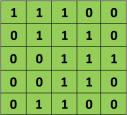
\includegraphics[height=1.5in]{pic/image_matrix.png}}%
\hspace{8pt}%
\subfigure[][]{%
\label{fig:ex3-bb}%
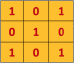
\includegraphics[height=1in]{pic/filter_matrix.png}}
\caption{\,\,\,\,\,\,\,\,\,\,Image matrix to and filter matrix for convolution operation
\subref{fig:ex3-aa} a 5 $\times$ 5 image matrix;
\subref{fig:ex3-bb} a 3 $\times$ 3 filter/kernel matrix}
\label{fig:convolution}
\end{figure}

\subsection{Non Linearity (ReLU)}
We perform a ReLU operation after every convolution. Rectified Linear Unit (ReLU) is an operation that simply replaces every negative pixel value in the feature map with zero. We write the ReLU function as $f(x) = max(0,x)$. The reason we use ReLU is to feed non-linearity into our CNN, since convolutional operation is a linear operation, ReLU helps to take care of non-linearity. Additionally, ReLU helps to speed up training of our CNN. Computation is very simple since we will be dealing with either $0$ or $1$ depending on $x$. There are other kinds of ReLU such as Noisy ReLUs\cite{Nair:2010:RLU:3104322.3104425}, Leaky ReLUSs\cite{Maas2013RectifierNI}, Parametric ReLUs\cite{7410480}, ELUs\cite{Clevert2015FastAA}, etc.

Noisy ReLUs introduces Gaussian noise in the rectified linear units, given below as
\[ f(x) = max(0, x + Y), \text{with} Y \sim N(0, \sigma(x))\]

Leaky ReLUs allow some positive values by multiplying input values less than zero by some fixed scalar. We express this operation as
\[ f(x) =
  \begin{cases}
    x, & \quad  \text{if } x \geq 0\\
    0.01x, & \quad \text{otherwise}
  \end{cases}
\]

Parametric ReLUs (PReLUs) further improves this idea by choosing a scalar that is learned during training just like any other neural network parameters. We express this operation as
\[ f(x) =
  \begin{cases}
    x, & \quad  \text{if } x \geq 0\\
    ax, & \quad \text{otherwise}
  \end{cases}
\]

Exponential linear units (ELUs) try to make the mean activations closer to zero which speeds up learning. It has been shown that ELUs can obtain higher classification accuracy than ReLUs.
\[ f(x) =
  \begin{cases}
    x, & \quad  \text{if } x \geq 0\\
    a(e^x - 1), & \quad \text{otherwise}
  \end{cases}
\]
$a$ is a hyper-parameter to be adjusted and $a \geq 0$ is a constraint.

\subsection{Pooling layer}
Pooling can be defined as the process of encoding and aggregating feature maps into a global feature vector \cite{cui2017cvpr}. The pooling layer reduces the spatial height and weight of the input by extracting only the important activations. This process helps to reduce computation and also helps to make the CNN translation invariant in terms of the convolution output. We have many kinds of pooling: max-pooling, average-pooling, sum-pooling, etc.

Max-pooling is performed by sliding a window (say, 2$\times$2 window) over the input and saving the maximum value of the elements withing the window space. Same process is applied for average-pooling and sum-pooling. However, for sum pooling we take the sum of all elements in that window and we take the average sum for average pooling. Max Pooling has shown better performance so far. Figure \ref{fig_maxpooling} shows an example of max pooling.

\subsection{Fully-Connected layer}
In this final layer we connect every neuron in the previous layer to neurons in the next layer. After going through several convolutional and pooling operations, the output is a high-level feature representation of the input image. The fully connected layer takes these high-level features as input and makes classification into one of the classes in the training dataset. Additionally, we use fully connected layer to learn the various feature combinations to help make better classifications. At the final layer of the fully connected is where the actual classification happens by implementing probabilities. We often use softmax activation function in the final output layer of the fully connected layer. We write the softmax activation function in equation \ref{fc_equation}.
\begin{equation}
    f_j(z) = \frac{e^{zj}}{\sum_{k}^{}e^{zk}}.
\label{fc_equation}
\end{equation}
Softmax function takes as input vector of arbitrary real-valued scores in $z$ and squashes it to vector of values between zero and one that sum up to one. These vector values represent the probability value of each of the classes to be present in the dataset. The highest vector value classifies the input image into it's corresponding class.

Apart from Softmax, Support Vector Machine (SVM) is another commonly used classifier. SVM seeks to find the best hyperplane that separates some given training data. We define the hyperplane in equation \ref{hyperplane_equation}.
\begin{equation}
    f(x) = \beta_{0} + \beta^{T} x
\label{hyperplane_equation}
\end{equation}
where $\beta$ is the \textit{weight} vector, $\beta_{0}$ as the \textit{bias} term and $x$ is the \textit{training examples}.

\begin{figure}[ht]
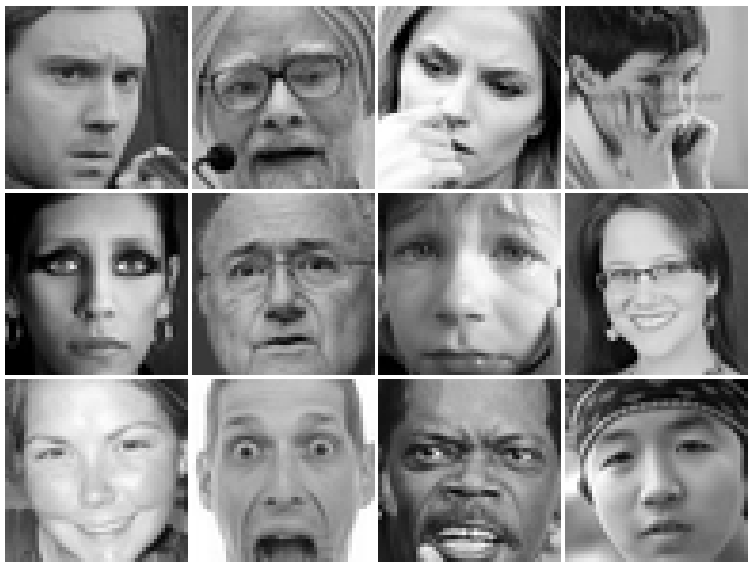
\includegraphics[width=5in]{pic/fer2013.png}
\caption{\,\,\,\,\,\,\,\,\,\,Examples of facial expression images from the FERC-2013 emotion database}
\label{fer2013_images}
\end{figure}

\begin{figure}[ht]
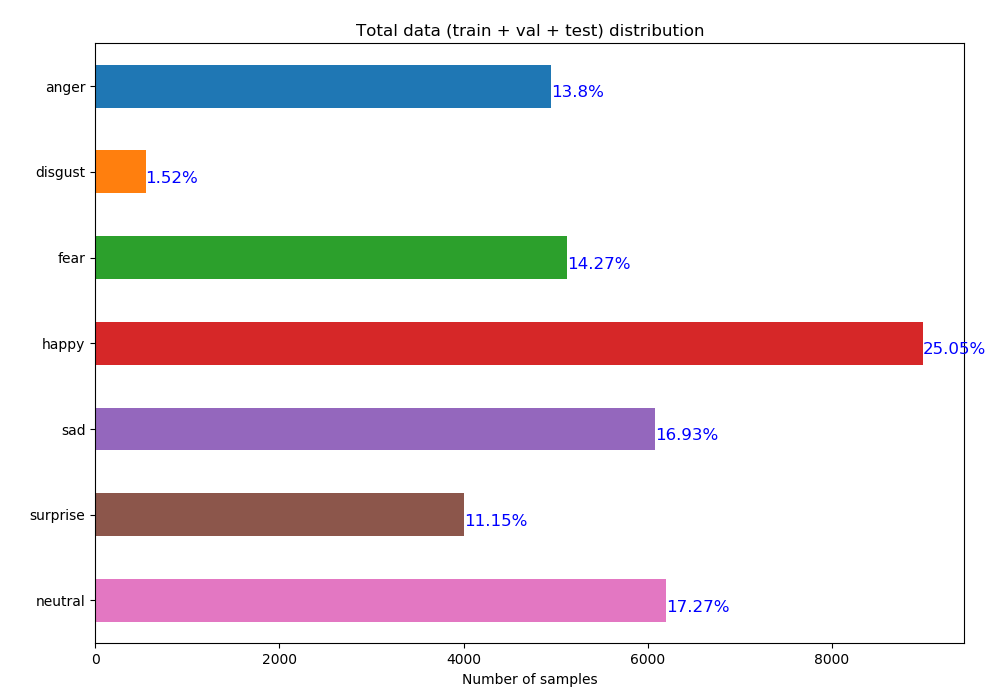
\includegraphics[width=5in]{pic/total_data_distribution.png}
\caption{\,\,\,\,\,\,\,\,\,\,FERC-2013 total sample distribution for Angry, Disgust, Fear, Happy, Sad, Surprise and Neutral emotion}
\label{fer2013_distribution}
\end{figure}

\begin{figure}[ht]
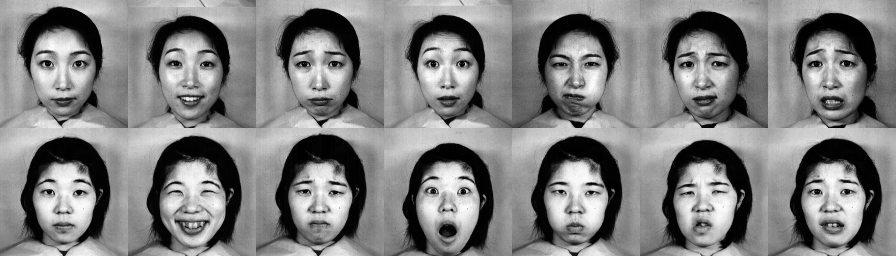
\includegraphics[width=5in]{pic/jaffe.png}
\caption{\,\,\,\,\,\,\,\,\,\,Examples of facial expression images from the Japanese Female Facial Expression (JAFFE) database.}
\label{jaffe_images}
\end{figure}

\begin{table}[ht]
\renewcommand{\arraystretch}{1}
\caption{\,\,\,\,\,Proposed Model Architecture containing approximately 474K parameters. \textit{DepthSep Conv2D} consists of two steps: first carrying out a depthwise spatial convolution and proceeded to perform a pointwise convolution to stack the output channels on top of each other. \textit{Max Pool} slide a $2 \times 2$ window size over the feature maps taking the maximum value in each local window region. \textit{Global Avg Pool} takes the global average of the feature maps. \textit{Softmax} is the classifier that outputs a 7 unit vector where each unit corresponds to one of the emotion categories.}
\label{model_arch}
\begin{center}
\begin{tabular}{|c|c|c|c|}
\hline
\textbf{Layer number} & \textbf{Layer name} & \textbf{Filter shape} & \textbf{output shape}\\ \hline
1 & DepthSep Conv2D & 3 x 3 x 1 x 32 & 48 x 48 x 32\\ \hline
2 & DepthSep Conv2D & 3 x 3 x 1 x 32 & 48 x 48 x 32\\ \hline
3 & DepthSep Conv2D & 3 x 3 x 1 x 32 & 48 x 48 x 32\\  \hline

4 & DepthSep Conv2D & 3 x 3 x 1 x 64 & 48 x 48 x 64\\ \hline
5 & DepthSep Conv2D & 3 x 3 x 1 x 64 & 48 x 48 x 64\\ \hline
6 & DepthSep Conv2D & 3 x 3 x 1 x 64 & 48 x 48 x 64\\  \hline

7 & Max Pool & 2 x 2 x 1 & 24 x 24 x 64\\ \hline

8 & DepthSep Conv2D & 3 x 3 x 1 x 92 & 24 x 24 x 92\\ \hline
9 & DepthSep Conv2D & 3 x 3 x 1 x 92 & 24 x 24 x 92\\ \hline
10 & DepthSep Conv2D & 3 x 3 x 1 x 92 & 24 x 24 x 92\\ \hline

11 & Max Pool & 2 x 2 x 1 & 12 x 12 x 92\\ \hline

12 & DepthSep Conv2D & 3 x 3 x 1 x 124 & 12 x 12 x 124\\ \hline
13 & DepthSep Conv2D & 3 x 3 x 1 x 124 & 12 x 12 x 124\\ \hline
14 & DepthSep Conv2D & 3 x 3 x 1 x 124 & 12 x 12 x 124\\ \hline

15 & Max Pool & 2 x 2 x 1 & 6 x 6 x 124\\ \hline

16 & DepthSep Conv2D & 3 x 3 x 1 x 124 & 6 x 6 x 124\\ \hline
17 & DepthSep Conv2D & 3 x 3 x 1 x 124 & 6 x 6 x 124\\ \hline
18 & DepthSep Conv2D & 3 x 3 x 1 x 124 & 6 x 6 x 124\\ \hline

19 & Max Pool & 2 x 2 x 1 & 3 x 3 x 124\\ \hline

20 & Global Avg Pool & Pool & 1 x 1 x 124\\ \hline
21 & Softmax & Classifier & 1 x 1 x 7\\ \hline

\end{tabular}
\end{center}
\end{table}

\begin{figure}[ht]
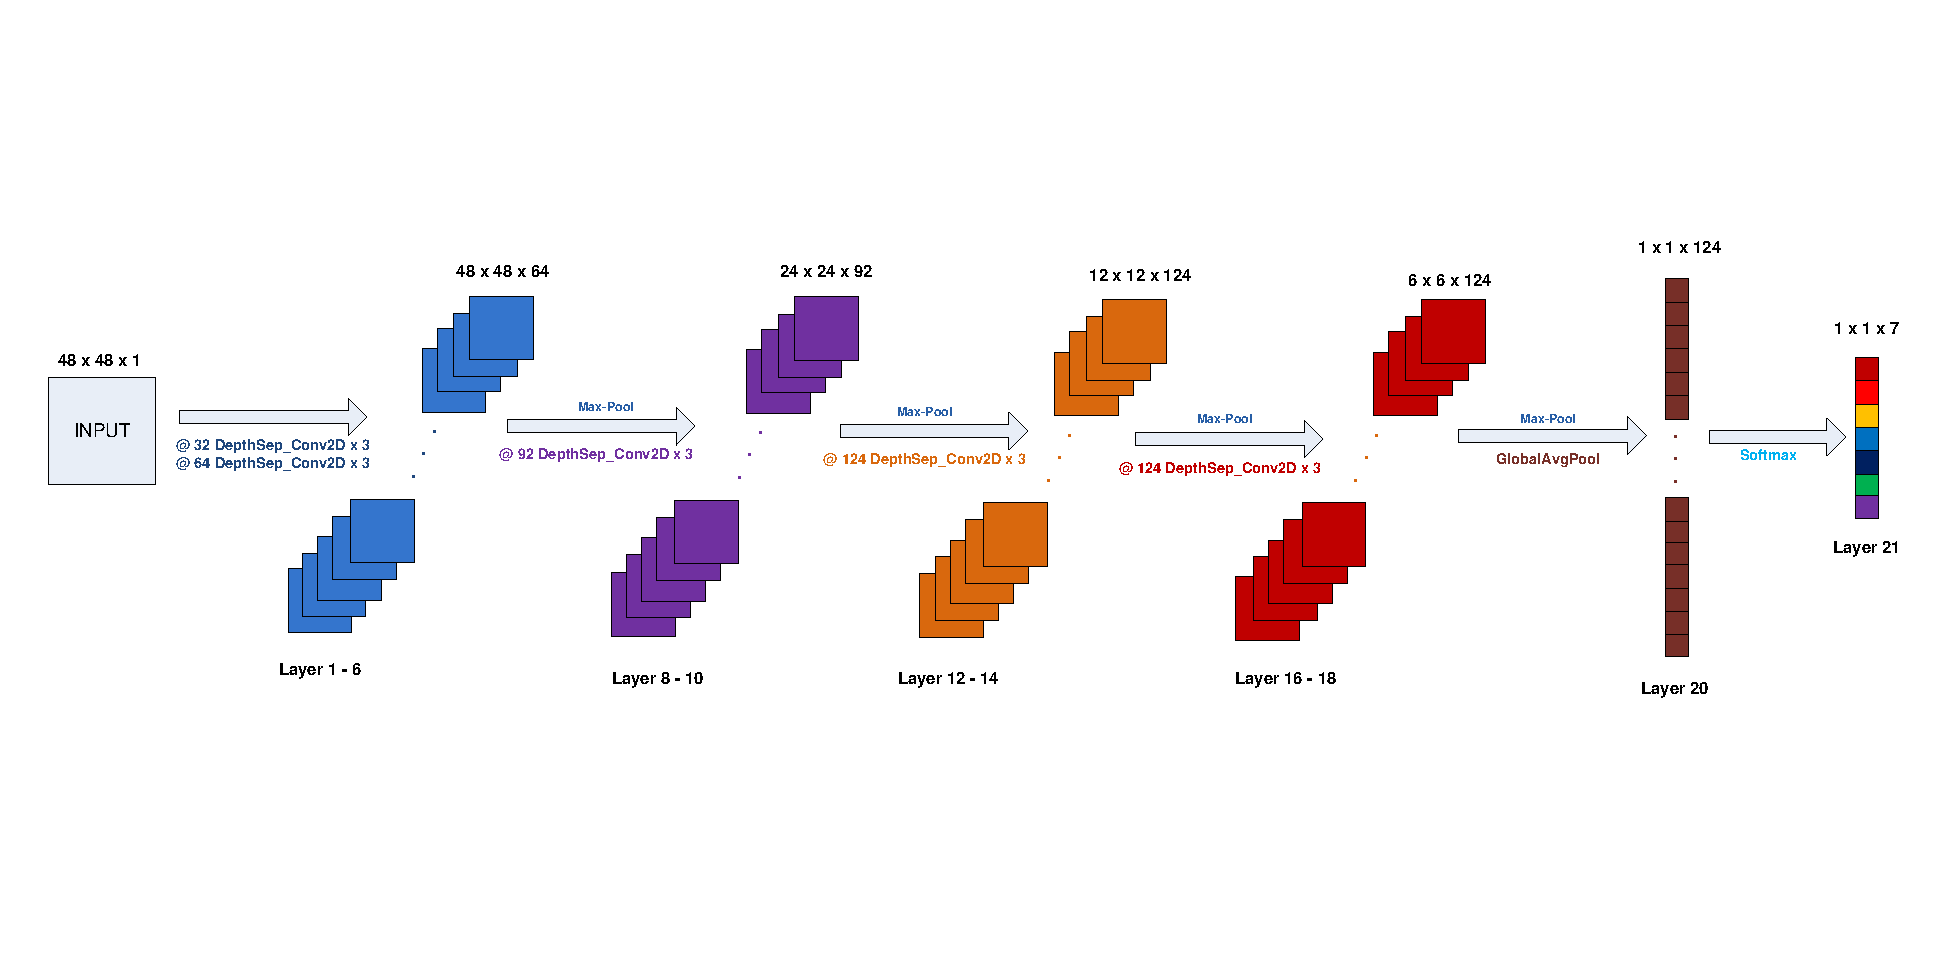
\includegraphics[width=6in]{pic/sequence_model_architecture.pdf}
\caption{\,\,\,\,\,\,\,\,\,\,The sequential view of the proposed model architecture and how input flows through the network.}
\label{sequence_model_arch}
\end{figure}

\section{Depthwise Separable Convolutions}\label{depthconve}
Depthwise Separable Convolution is a type of convolution that splits the convolution operation into two steps. It transforms standard convolution by factorizing into a depthwise convolution and a $1 \times 1$ standard convolution termed as pointwise convolution. Depthwise separable convolutions have been used successfully in recent deep neural network models such as MobileNets\cite{DBLP:journals/corr/HowardZCKWWAA17}, Xception\cite{DBLP:journals/corr/Chollet16a} and Effnet\cite{8451339}.

In the first operation for depthwise convolution, given an RGB input image of spatial dimension $12 \times 12 \times 3$, we use 3 filters of shape $5 \times 5\times 1$. Each $5 \times 5\times 1$ filter performs convolution on 1 channel of the input image, resulting in scalar products of every 25 pixel group with an output shape of $8\times8\times1$. We stack these output images together to form a $8\times8\times3$ image.

In the second operation, we perform pointwise convolution, we use a $1\times1\times n$ filter to perform convolution across all channels. The filter will have the same number of $n$ channels as the input image. In our example, we will use a $1\times1\times3$ filter to perform convolution on our $8\times8\times3$ image. At this point, we use 32 filters of size $1\times1\times3$ to perform convolution on our input image that output a $8\times8\times1$ image for each of our 32 filter of size $1\times1\times3$. We stack all the output together to get our final output image of shape $8\times8\times32$ just like what a standard convolution will achieve.

Depthwise separable convolution provides three main advantages over regular convolutions:
\begin{enumerate}
    \item Depthwise separable convolutions are less prone to overfitting because they have fewer parameters compared to regular convolutions
    \item Because they have fewer parameters, computation cost is less and thus speeds up the model execution and time
    \item Depthwise separable convolution is more attractive for real-time applications and running on mobile devices because of efficiency
\end{enumerate}

\subsection{Regular vs. Depthwise Separable Convolutions: Computational Cost}
We define the following notations. Let:
    \[w, h = \text{spatial width, spatial height}\]
    \[I_w, I_h = \text{input image width, input image height} \]
    \[F_w, F_h = \text{filter width, filter height}\]
    \[C_i = \text{number of input channels}\]
    \[C_o = \text{number of output channels}\]
Let us assume same padding for every convolution operation such that spatial input size is the same as spatial output size and every filter is a 3D tensor of shape $F_w \times F_h \times C_{in}$

For regular convolution, parameter computation at each position of the input image can be given as $F_w \times F_h \times C_i$. Performing convolution over the whole input image makes the computation cost $F_w \times F_h \times C_i \times I_w \times I_h$. Considering all output channels $C_o$, our final computational cost becomes $F_w \times F_h \times C_i \times I_w \times I_h \times C_i$

For depthwise separable convolution, $F_w \times F_h \times C_i \times I_w \times I_h$ total cost is required in the depthwise operation. In the pointwise operation, we need $I_w \times I_h \times C_o$ cost. Hence, total computational cost becomes $(F_w \times F_h \times C_i \times I_w \times I_h) + (I_w \times I_h \times C_o)$.

For further illustration, let's consider the following example. Let's assume $I_w = 128, I_h = 128, F_w = 3, F_h = 3, C_o = 16$ \\
\textbf{For regular convolution:} \\
parameters:
\[3 \times 3 \times 16 = 432\]
computation cost:
\[3 \times 3 \times 3 \times 128 \times 128 \times 16 = \sim7e6\]
\textbf{For depthwise separable convolution:}\\
parameters:
\[3 \times 3 + 16 = 75 \]
computation cost:
\[(3 \times 3 \times 3 \times 128 \times 128 \times) + (128 \times 128 \times 3 \times 16) = \sim1.2e6 \]

We can evidently see the computational cost advantages depthwise separable convolution have over regular convolution. In the example above, depthwise separable convolution have about $\sim5.5e6$ fewer parameters than regular convolution for the same convolutional operation.

\begin{figure}[ht]
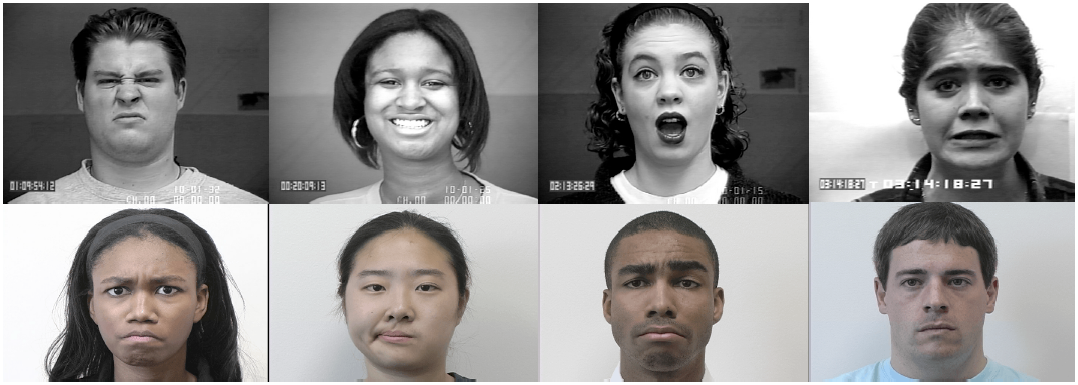
\includegraphics[width=5in]{pic/ck+.PNG}
\caption{\,\,\,\,\,\,\,\,\,\,Examples of images from the CK+ database. The top four horizontal grayscale images are taken from the original CK database and the other four horizontal RGB images at the bottom are taken from the CK+ dataset. All together we have 8 emotions and 30 AUs. Examples of the Emotion and AU labels
are: (a) Disgust - AU 1+4+15+17, (b) Happy - AU 6+12+25, (c) Surprise - AU 1+2+5+25+27, (d) Fear - AU 1+4+7+20, (e) Angry - AU 4+5+15+17, (f) Contempt - AU 14, (g) Sadness - AU 1+2+4+15+17, and (h) Neutral - AU0. Source: Lucey et al.\cite{5543262}}
\label{CK+_images}
\end{figure}

\section{Summary}
In this chapter we presented the theoretical basics underlying this research work. We started by discussing what machine learning is and the types or forms of machine learning techniques in existence. We went further to discuss in details one example of the techniques in machine learning, deep learning. Furthermore, we discussed one popular type of deep learning method called convolutional neural network. Finally, we took a look at a type of convolutional neural network called depthwise separable convolutions and analyzed the computation cost of a regular convolution vs depthwise separable convolution.

\chapter{\,\,\,\,\,\textbf{Proposed Method and Experiments}}
In this section, we will describe our proposed CNN model based on depthwise separable convolution for facial expression recognition problem and provide details of the layers that constituents the model. This chapter also presents the computation cost of the model and describes the various experiments conducted.

\section{Model Architecture}
Our proposed model structure is a pure convolutional network (i.e. without any fully-connected layer) that is based on depthwise separable convolutions as explained in section \ref{depthconve}. All depthwise separable layers perform \textit{same convolution} with a filter size of $3 \times 3 \times 1$ and a \textit{depth-multiplier} value of $1$ shifting by $1$ stride. We use ReLU\cite{7410480} activation function in all the separable convolutional layers to help us avoid the vanishing gradient problem\cite{5264952}. All depthwise separable convolutional layers are followed by a batch normalization operation\cite{DBLP:journals/corr/IoffeS15} to normalize the output in each layer in order to avoid varying distributions of the features across the training and test data. For our model to generalize well on unseen data and avoid overfitting on the training data, we apply dropout\cite{JMLR:v15:srivastava14a} as our regularization method in the last three depthwise separable convolutional layers. We apply Max-Pooling of window size $2 \times 2$ and stride $1$ after the $6^{th}$, $9^{th}$, $12^{th}$, and $15^{th}$ depthwise separable convolutional layers in order to down sample input flowing through the network. Instead of the traditional fully connected layer, we output the spatial average of the learned feature maps from the last depthwise separable convolutional layer via a global average pooling layer \cite{DBLP:journals/corr/LinCY13}; and the output feature vector is fed into the softmax layer for classification.  In summary, the entire network contains only $474K$ parameters with 15 separable convolutional layers and four pooling layers. Table \ref{model_arch} shows details of our proposed model architecture. Figure \ref{sequence_model_arch} shows the architecture of our proposed model.

The model starts by feed forwarding training examples through a continuous $6$ depthwise separable convolution layers. The first three depthwise separable layers have $32$ filters each. Each of the first $3$ depthwise separable layers takes in input shape $48 \times 48 \times 1$ and outputs $48 \times 48 \times 32$ after depthwise separable convolution operation. The next three depthwise separable layers have $64$ filters each. Apart from the $4^{th}$ layer which takes an input shape $48 \times 48 \times 32$, the $5^{th}$ and $6^{th}$ layers receive input shape $48 \times 48 \times 64$ and outputs $48 \times 48 \times 64$.

After the first six depthwise separable layers, we perform the first max-pooling at layer 7 to down-sample the feature map dimension from $48 \times 48 \times 64$ to $24 \times 24 \times 64$. The $8^{th}, 9^{th}$ and $10^{th}$ depthwise separable layers have $92$ filters each. The $8^{th}$ depthwise separable layer takes in input shape $24 \times 24 \times 64$ and output $24 \times 24 \times 92$. The output from the $8^{th}$ layer is fed to the $9^{th}$ layer; the $9^{th}$ layer's output is then fed to the $10^{th}$ layer to produce output shape $24 \times 24 \times 92$ after depthwise separable convolution operation.

After the $10^{th}$ depthwise separable layer, we perform the second max-pooling at layer 11 to further down-sample the feature map dimension from $24 \times 24 \times 92$ to $12 \times 12 \times 92$. The $12^{th}, 13^{th}$ and $14^{th}$ depthwise separable layers have $124$ filters each. The $12^{th}$ depthwise separable layer takes in input shape $12 \times 12 \times 92$ and outputs $12 \times 12 \times 124$. The output from the $12^{th}$ layer is fed to the $13^{th}$ layer; the $13^{th}$ layer's output is then fed to the $14^{th}$ layer to produce output shape $12 \times 12 \times 124$ after depthwise separable convolution operation.

After the $14^{th}$ depthwise separable layer, we perform the third max-pooling at layer 15 to down-sample the feature map dimension furthermore from $12 \times 12 \times 124$ to $6 \times 6 \times 124$. The $16^{th}, 17^{th}$ and $18^{th}$ depthwise separable layers also have $124$ filters each. All three layers ($16^{th}, 17^{th}$ and $18^{th}$) take in input shape $6 \times 6 \times 124$. The output from the $16^{th}$ layer is fed to the $17^{th}$ layer; the $17^{th}$ layer's output is then fed to the $18^{th}$ layer to produce output shape $6 \times 6 \times 124$ after depthwise separable convolution operation.

After the $18^{th}$ depthwise separable layer, we perform the final max-pooling at layer 19 to down-sample the feature map from $6 \times 6 \times 124$ to a final dimension of $3 \times 3 \times 124$. In CNN architectures, it has been the tradition to use fully connected layers to learn feature combinations from the last convolution layer. Instead, we feed the output from the last depthwise separable convolution layer ($18^{th}$ layer) to a global average pooling operation at layer $20$ in order to combine all the various features learned from the convolution operations. At the global average pooling layer, we produce single feature map for every corresponding class of our facial emotion recognition task by computing the average of each feature map. We use Global Average Pooling instead of the traditional fully connected layers because of the following reasons:
\begin{itemize}
    \item \textbf{Confidence:} global average pooling is increasingly local to the convolution structure by implementing correspondences between feature maps and classes. In this way, the feature maps can be effortlessly translated as classes certainty maps.
    \item \textbf{Overfitting:} fully connected layers are highly parameterized and are prone to overfitting. Global average pooling do not involve any parameter optimization, hence, there is no potential of causing overfitting in this layer.
    \item \textbf{Robustness: } also, global average pooling computes the spatial information from the feature maps, therefore it is very robust to spatial interpretations of the input.
\end{itemize}
The output after the global average pooling is fed to the final layer ($21^{th}$), that is the softmax layer for classification. The softmax layer outputs a vector of shape $1 \times 1 \times 7$ with each vector value corresponding to one of the seven facial emotion classes.

\begin{comment}
\begin{table}[ht]
\renewcommand{\arraystretch}{1.3}
\caption{\,\,\,\,\,Model Architecture for JAFFE dataset containing approximately 120K parameters}
\label{small_model_arch}
\begin{center}
\begin{tabular}{|c|c|c|c|}


\hline
\textbf{Layer number} & \textbf{Layer name} & \textbf{Filter shape} & \textbf{output shape}\\ \hline

1 & DepthSep Conv2D & 3 x 3 x 1 x 32 & 48 x 48 x 32\\ \hline
2 & DepthSep Conv2D & 3 x 3 x 1 x 32 & 48 x 48 x 32\\ \hline
3 & DepthSep Conv2D & 3 x 3 x 1 x 32 & 48 x 48 x 32\\  \hline

4 & DepthSep Conv2D & 3 x 3 x 1 x 64 & 48 x 48 x 64\\ \hline
5 & DepthSep Conv2D & 3 x 3 x 1 x 64 & 48 x 48 x 64\\ \hline
6 & DepthSep Conv2D & 3 x 3 x 1 x 64 & 48 x 48 x 64\\  \hline

7 & Max Pool & 2 x 2 x 1 & 24 x 24 x 64\\ \hline

8 & DepthSep Conv2D & 3 x 3 x 1 x 92 & 24 x 24 x 92\\ \hline
9 & DepthSep Conv2D & 3 x 3 x 1 x 92 & 24 x 24 x 92\\ \hline
10 & DepthSep Conv2D & 3 x 3 x 1 x 92 & 24 x 24 x 92\\ \hline

11 & Global Avg Pool & Pool & 1 x 92\\ \hline
12 & Softmax & Classifier & 1 x 1 x 7\\ \hline
\end{tabular}
\end{center}
\end{table}
\end{comment}

\section{Experiments}
We experiment our model using supervised learning techniques. That it, we expose the model to large amount of data and we allow it to learn the optimal features and parameters for the underlined task.

\begin{figure}[ht]
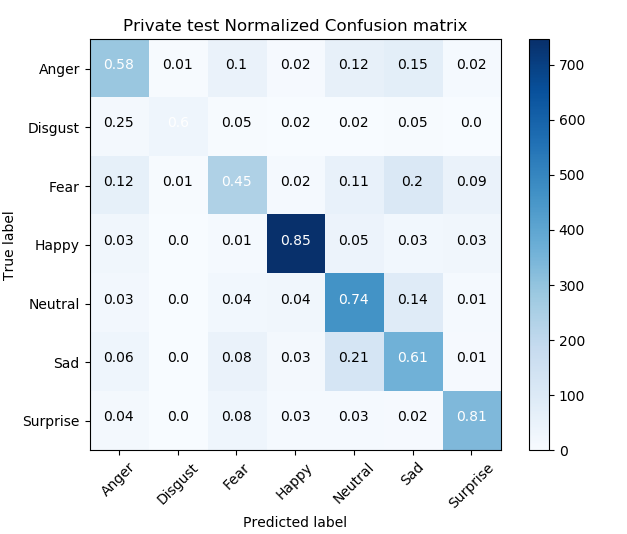
\includegraphics[width=5in]{pic/FER-2013_private_test_CM_normalzed.png}
\caption{\,\,\,\,\,\,\,\,\,\,Normalized confusion matrix on model test accuracy for FERC-2013 private test.}
\label{fig_ferpr_cm_scores}
\end{figure}

\begin{figure}[ht]
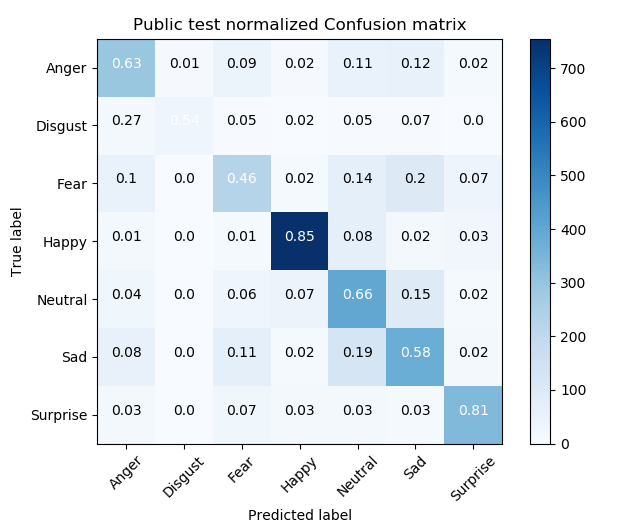
\includegraphics[width=5in]{pic/FER-2013_public_test_CM_normalzed.png}
\caption{\,\,\,\,\,\,\,\,\,\,Normalized confusion matrix on model test accuracy for FERC-2013 public test}
\label{fig_ferpub_cm_scores}
\end{figure}

\begin{figure}[ht]
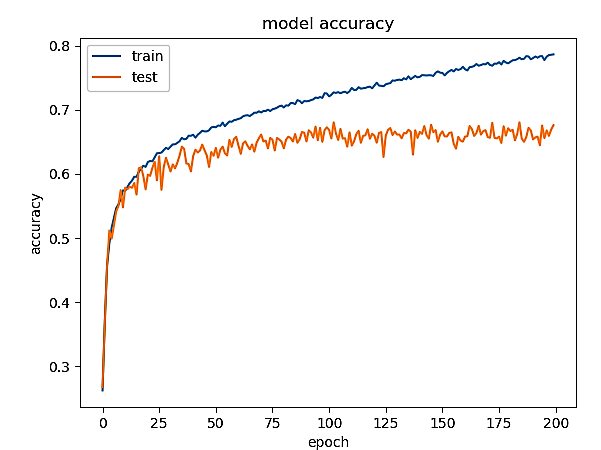
\includegraphics[width=5in]{pic/model_accuracy_fer.png}
\caption{\,\,\,\,\,\,\,\,\,\,Model training and validation accuracy.}
\label{fer_accuracy}
\end{figure}

\begin{figure}[ht]
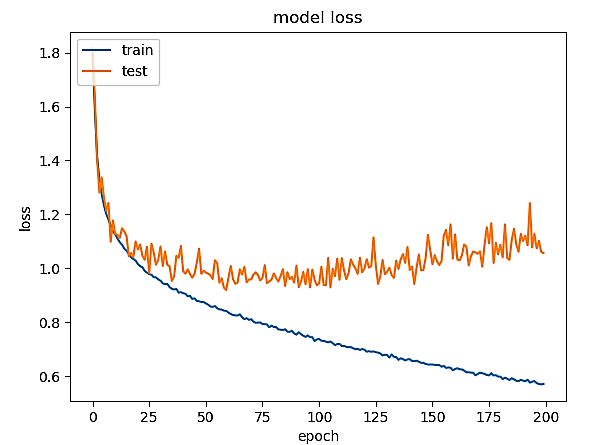
\includegraphics[width=5in]{pic/model_loss_fer.png}
\caption{\,\,\,\,\,\,\,\,\,\,Model training and validation loss}
\label{fer_loss}
\end{figure}

\subsection{Datasets}
We experiment our proposed model on three famous dataset for the task of facial expression recognition. The three datasets are FERC-2013, JAFFE database and CK+ database.

\subsubsection{FERC-2013}
FERC-2013 was prepared by Pierre-Luc Carrier and Aaron Courville and used by Kaggle during the Challenges in Representation Learning: Facial Expression Recognition Challenge in 2013. The dataset is made up of $48\times48$ pixel grayscale images of faces categorized into the seven emotion classes (0=Angry, 1=Disgust, 2=Fear, 3=Happy, 4=Sad, 5=Surprise, 6=Neutral). The dataset contains uneven distribution of the emotion classes with happy emotion containing the highest with 25.05\%, followed by neutral emotion with 17.27\%, followed by sad emotion with 16.93\%, followed by fear emotion with 14.27\%, followed by anger with 13.8\%, followed by surprise with 11.15\% and disgust emotion contains the smallest examples with only 1.52\%.  All the faces contained in the dataset images are positioned in such a way that it is centered and covers bigger portions of the entire image. The \textit{train.csv} file has two columns, \textit{emotion} and \textit{pixels}. The \textit{emotion} column is made up of digit code inclusively spanning from 0 to 6 corresponding to one of the seven emotions. The \textit{pixels} are made up of strings enclosed in quotes for each image. The strings contain the pixel values in row major order separating each pixel value with a space. The \textit{test.csv} file houses only the the `pixel' values for each test image. There contain 35,896 total samples with 28,709 training samples, 3,589 samples for public test and another 3,589 samples for private test.  Examples of facial expression images from the FERC-2013 emotion database are shown in Figure \ref{fer2013_images}.

\subsubsection{Japanese Female Facial Expression}
% We validate the effectiveness of our proposed method on FERC-2013 and JAFFE database in order to appropriately generalize our model for facial expression recognition.
The Japanese Female Facial Expression (JAFFE) database contains $256\times256$ pixel 213 grayscale images of the seven facial expressions posed by 10 Japanese female models. Facial expression images were coded using a multi-orientation, multi-resolution set of Gabor filters which were topographically ordered and arranged pretty much with the face. The similarity space
obtained from this representation was crosschecked with one obtained from semantic ratings of the images by human observers. The Gabor representation demonstrated a notable degree of psychological credibility, a design feature which may be important for human-computer interfaces. Examples of facial expression images from the Japanese Female Facial Expression (JAFFE) database are shown in Figure \ref{jaffe_images}.

\subsubsection{Extended Cohn-Kanade Dataset}
The Extended Cohn-Kanade Dataset (CK+) dataset is a built on the work done by T. Kanade et al.\cite{ck_840611}. In the work done by T. Kanade et al.\cite{ck_840611}, they presented a sequence of 2105 images obtained from 128 adult subjects of different ethnicity. The subjects expressed the various emotions by acting the multiple tokens of many basic Facial Action Coding System (FACS)\cite{ekman_facs} action units. The Extended Cohn-Kanade Dataset (CK+) dataset increased the sequence of images by $22\%$ and the also increased the number of adult subjects by $27\%$. All label expressions for each sequence was fully based on FACS coding. Also, CK+ dataset added non-posed sequences for many kinds of smiles and their corresponding metadata. Examples of facial expression images from the CK+ dataset are shown in Figure \ref{CK+_images}

\begin{table}[ht]
\renewcommand{\arraystretch}{1.3}
\caption{\,\,\,\,\,Model accuracy for public test on Precision, Recall and F1-score for FERC-2013 dataset}
\label{table_fer2013_scores_public}
\begin{center}
\begin{tabular}{|c|c|c|c|c|}

\hline
 & Precision & Recall & F1-score & Support\\ \hline

Anger & 0.63 & 0.63 & 0.63 & 467\\ \hline
Disgust & 0.71 & 0.54 & 0.61 & 56\\ \hline
Fear & 0.56 & 0.46 & 0.51 & 496\\ \hline
Happy & 0.90 & 0.85 & 0.87 & 890\\ \hline
Neutral & 0.55 & 0.66 & 0.60 & 607\\ \hline
Sad & 0.58 & 0.58 & 0.58 & 653\\ \hline
Surprise & 0.78 & 0.81 & 0.79 & 415\\ \hline

\textbf{avg / total} & \textbf{0.68} & \textbf{0.68} & \textbf{0.68} & \textbf{3584}\\ \hline

\end{tabular}
\end{center}
\end{table}

\subsection{Model Training}
For training and testing we implemented our network architecture using Keras Deep Learning library\footnote{Keras is a high-level neural networks API, written in Python - https://keras.io/}. We ran the experiments on independent streams on GPU using NVIDIA CUDA parallel computing platform. We conduct training on FERC-2013 dataset, JAFFE dataset and CK+ dataset. For all datasets, we trained for 200 epochs. In order to make our model more robust and speed up training, we implemented the following real-time data augmentation and preprocessing during training:
\begin{itemize}
 \item rescaling images to 1./255 in order to transform every pixel value from range [0,255] to [0,1]
 \item image shearing clockwise value of 0.2
 \item  random zoom range of 40
 \item  image width and height shifting of 0.2
 \item random horizontal flipping
 \item image cropping of 48 x 48
 \item converting all RGB images to grayscale
\end{itemize}
We maintained a batch size of 32 across all datasets to feed input into the network. We trained the network using Adam Optimizer \cite{DBLP:journals/corr/KingmaB14} with learning rate of 0.001 for all datasets. Training results are presented in chapter 4. Finally, we implemented our model with OpenCV on an Intel Dual Core i3-7100U 2.4GHz Processor laptop in real-time by connecting a live video stream to a face detector to feed images to our trained model to recognise the 7 basic emotions.

\begin{table}[ht]
\renewcommand{\arraystretch}{1.3}
\caption{\,\,\,\,\,Model accuracy for private test on Precision, Recall and F1-score for FERC-2013 dataset}
\label{table_fer2013_scores_private}
\begin{center}
\begin{tabular}{|c|c|c|c|c|}

\hline
 & Precision & Recall & F1-score & Support\\ \hline

Anger & 0.63 & 0.58 & 0.61 & 491\\ \hline
Disgust & 0.73 & 0.60 & 0.66 & 55\\ \hline
Fear & 0.59 & 0.45 & 0.51 & 528\\ \hline
Happy & 0.92 & 0.85 & 0.88 & 874\\ \hline
Neutral & 0.61 & 0.74 & 0.67 & 626\\ \hline
Sad & 0.54 & 0.61 & 0.58 & 594\\ \hline
Surprise & 0.77 & 0.81 & 0.79 & 416\\ \hline

\textbf{avg / total} & \textbf{0.69} & \textbf{0.69} & \textbf{0.69} & \textbf{3584}\\ \hline
\end{tabular}
\end{center}
\end{table}

\section{Summary}
This chapter presents the proposed model architecture and the various experiments conducted. Also, the chapter presents all the technical details for the model training on three different datasets.

\chapter{\,\,\,\,\,\textbf{Results and Analysis}}\label{chp4}
In this chapter we present the results and analysis of the experiments on the three dataset: FERC-2013 dataset, JAFFE dataset and CK+ dataset. We also present the results metrics used to evaluate the model performance.
\section{Results Metrics}
We evaluated the model by calculating the accuracy, precision, recall, f1-score and confusion matrix\cite{FAWCETT2006861} for all three datasets. We perform the calculations based on the following parameters: True Positives (TP), True Negatives (TN), False Positives (FP) and False Negatives (FN). TP are the correctly predicted positive values, thus, when target label is `yes' and the predicted label is also `yes'. TN are correctly predicted negative values, thus, when target label is `no' and the predicted label is also `no'. FP are the predicted values where target label is `no' but the predicted label is `yes'. FN are the values where target label is `yes' but the predicted label is `no'.

We define accuracy as simply the ratio of correctly classified samples to the total test samples. Accuracy of the model was calculated according to formula \ref{accuracy_equation}.
\begin{equation}
Accuracy=\frac{TP + TN}
 {TP + FP + FN + TN}
 \label{accuracy_equation}
\end{equation}

Precision is the ratio of correctly classified positive samples to the total classified positive samples. Intuitively, precision relates to false positive rate, in that, the lower the false positives the higher our precision. Precision of the model was calculated according to formula \ref{precision_formula}.
\begin{equation}
Precision=\frac{TP}
 {TP + FP}
 \label{precision_formula}
\end{equation}

Recall or Sensitivity is the ratio of correctly classified positive samples to all samples belonging to the actual class. Recall of the model was calculated according to formula \ref{recall_formula}.
\begin{equation}
Recall=\frac{TP}
 {TP + FN}
\label{recall_formula}
\end{equation}

F1-score is simply the weighted average of Precision and Recall. In this sense, F1-score considers both the false positives and false negatives. We calculated for F1-score because the three datasets (FERC-2013, JAFFE and CK+) have uneven distribution of class samples. This means false positives and false negative have different cost contribution to the model accuracy. F1-score of the model was calculated according to formula \ref{f1-score_formula}.
\begin{equation}
F1-score=2\frac{Precision \times Recall}
 {Precision + Recall}
\label{f1-score_formula}
\end{equation}

For all confusion matrices, the major diagonal of the matrix contains the correctly predicted labels, thus $TP$ and $TN$ values. The values outside the major diagonal represent the wrongly predicted labels. The values above the major diagonal are the $FP$ values.

\begin{table}[ht]
\renewcommand{\arraystretch}{1.3}
\caption{\,\,\,\,\,Model test accuracy on Precision, Recall and F1-score for JAFFE dataset}
\label{table_jaffe_scores}
\begin{center}
\begin{tabular}{|c|c|c|c|c|}

\hline
 & Precision & Recall & F1-score & Support\\ \hline

Anger & 0.82 & 1.00 & 0.90 & 9\\ \hline
Disgust & 1.00 & 0.78 & 0.88 & 9\\ \hline
Fear & 0.91 & 1.00 & 0.95 & 10\\ \hline
Happy & 1.00 & 1.00 & 1.00 & 10\\ \hline
Neutral & 0.71 & 1.00 & 0.83 & 10\\ \hline
Sad & 0.83 & 0.50 & 0.62 & 10\\ \hline
Surprise & 1.00 & 0.90 & 0.95 & 10\\ \hline

\textbf{avg / total} & \textbf{0.90} & \textbf{0.88} & \textbf{0.88} & \textbf{68}\\ \hline
\end{tabular}
\end{center}
\end{table}

\begin{figure}[ht]
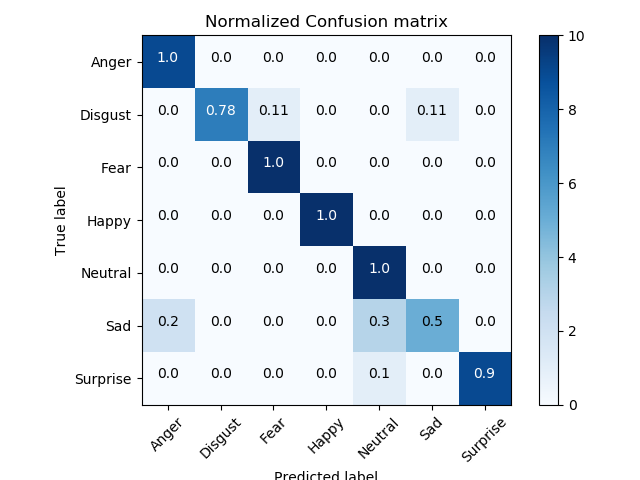
\includegraphics[width=5in]{pic/JAFFE_CM_normalized.png}
\caption{\,\,\,\,\,\,\,\,\,\,Normalized confusion matrix on model test accuracy for JAFFE dataset}
\label{fig_jaffe_cm_scores}
\end{figure}

\section{Analysis}
For the FERC-2013 dataset, the model achieved 68\% on precision, recall and f1-score on the public test examples. During the private test, the model obtained 69\% performance on precision, recall and f1-score. Table \ref{table_fer2013_scores_public} and Table \ref{table_fer2013_scores_private} shows the model accuracy details on the public and private test respectively. It was observed that the model performed worst in recognizing fear and sad expressions. From the confusion matrix in Figure \ref{fig_ferpr_cm_scores} and Figure \ref{fig_ferpub_cm_scores}, the model often confused fear for sad and also confused sad for neutral and anger. We also observed from the dataset that fear and sad expressions exhibits similar facial movements with the forehead been squeezed and the mouth tightly closed. Additionally, many sad expression samples looked similar to neutral and anger, both expressions have the mouth closed and steady facial contour. However, among the seven emotions, the model performance on happy emotion was the highest, obtaining up to 87\% and 88\% for public and private test respectively. This result can be explained by observing the total sample distribution of the emotion classes in the dataset as shown in Figure \ref{fer2013_distribution}. The happy emotion contains the largest samples (25.05\%) among all the other emotion classes. Consequently, the model is exposed to larger number of happy emotion samples and learns more optimal features to distinguish happy emotion from other emotions. In order to avoid the model memorizing the training data and not generalization well on unseen data, we stop training after 200 epochs. As shown in Figure \ref{fer_accuracy}, the model did not significantly improve the validation accuracy from epoch 150. This is evident from training and validation loss as shown in Figure \ref{fer_loss}, the validation loss did not further reduce after epoch 150. Training on FERC-2013 dataset spanned a period of approximately 7 hours.

For the JAFFE dataset, the model achieved 88\% accuracy on test samples. From Table \ref{table_jaffe_scores}, we can see that the only emotion category the model obtained a 100\% f1-score is the \textit{happy} emotion. Taking a closer look at the image samples in the JAFFE dataset, we observed that \textit{happy} emotion examples are quite distinct from the other emotion examples. The \textit{happy} emotion samples do not have the forehead and mouth region tightly squeezed like most other emotion expressions (fear, sad, disgust and anger). Hence, the model is able to learn these distinct features to obtain the 100\% f1-score for the \textit{happy} emotion. From the generated confusion matrix in Figure \ref{fig_jaffe_cm_scores}, we also observed that the model often confused fear and sad for disgust. Taking a look at the training samples , all the 3 expressions are very similar with the forehead and mouth region (sad expression) tightly squeezed. 
% \begin{table}[ht]
% \renewcommand{\arraystretch}{1.3}
% \caption{Model test accuracy on Precision, Recall and F1-score for CK+ dataset. The first column contains the seven emotion classes (Anger, Contempt, Disgust, Fear, Happy, Sadness and Surprise), the second, third and fourth column contain the Precision, Recall, F1-score for each emotion respectively. The fifth column contains the number of samples observed for each emotion class. The last row contains the averaged Precision, Recall, F1-score and the total samples observed.}
% \label{table_ck+_scores}
% \begin{center}
% \begin{tabular}{|c|c|c|c|c|}

% \hline
%  & Precision & Recall & F1-score & Support\\ \hline

% Anger & 0.20 & 0.07 & 0.11 & 14\\ \hline
% Contempt & 0.40 & 0.40 & 0.40 & 5\\ \hline
% Disgust & 0.17 & 0.17 & 0.17 & 18\\ \hline
% Fear & 0.11 & 0.12 & 0.12 & 8\\ \hline
% Happy & 0.32 & 0.30 & 0.31 & 20\\ \hline
% Sadness & 0.12 & 0.25 & 0.16 & 8\\ \hline
% Surprise & 0.32 & 0.32 & 0.32 & 25\\ \hline

% \textbf{avg / total} & \textbf{0.24} & \textbf{0.23} & \textbf{0.23} & \textbf{98}\\ \hline
% \end{tabular}
% \end{center}
% \end{table}

\begin{table}[ht]
\renewcommand{\arraystretch}{1.3}
\caption{\,\,\,\,\,Model test accuracy on Precision, Recall and F1-score for CK+ dataset}
\label{table_ck+_scores}
\begin{center}
\begin{tabular}{|c|c|c|c|c|}

\hline
 & Precision & Recall & F1-score & Support\\ \hline

Anger & 1.00 & 1.00 & 1.00 & 14\\ \hline
Contempt & 1.00 & 0.80 & 0.89 & 5\\ \hline
Disgust & 1.00 & 1.00 & 1.00 & 18\\ \hline
Fear & 0.89 & 1.00 & 0.94 & 8\\ \hline
Happy & 1.00 & 1.00 & 1.00 & 20\\ \hline
Sadness & 1.00 & 1.00 & 1.00 & 8\\ \hline
Surprise & 1.00 & 1.00 & 1.00 & 24\\ \hline

\textbf{avg / total} & \textbf{0.99} & \textbf{0.99} & \textbf{0.99} & \textbf{98}\\ \hline
\end{tabular}
\end{center}
\end{table}

\begin{figure}[ht]
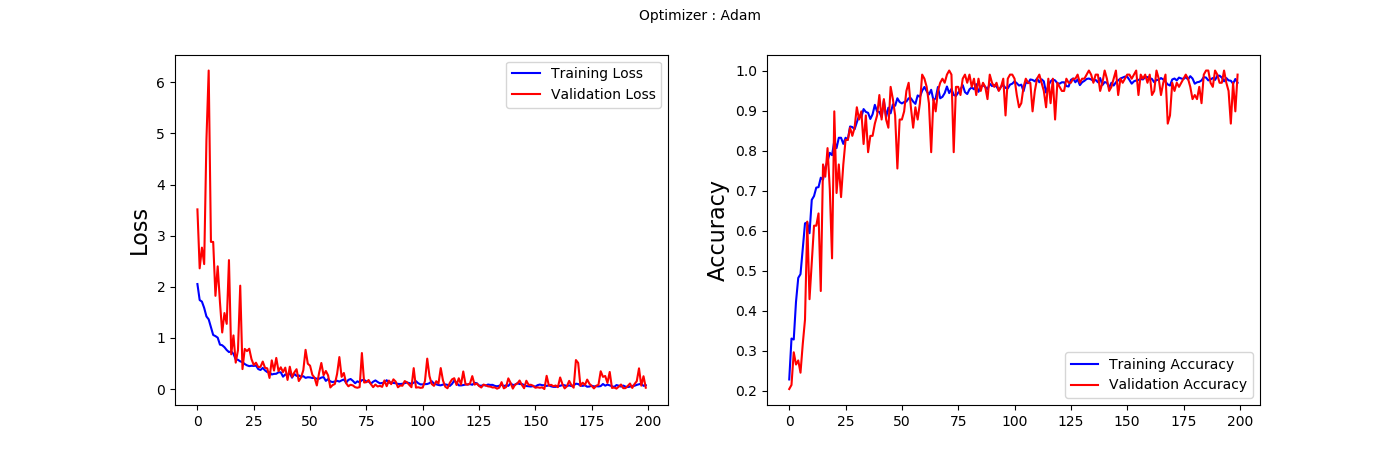
\includegraphics[width=6.5in]{pic/XK+_accuracy_and_loss.png}
\caption{\,\,\,\,\,\,\,\,\,\,Model training and validation accuracy and loss on CK+ dataset. The graph on the left is the accuracy increase for 200 epochs and the graph on the right is the loss reduction for 200 epochs}
\label{ck+accuracy_loss}
\end{figure}

For CK+ dataset, our model achieved $99\%$ test accuracy and $0.03941$ for test loss. We present details accuracy for each of the seven emotion category in Table \ref{table_ck+_scores}. As shown in Figure \ref{ck+_cm}, the model obtained prediction accuracy up to $100\%$ for all emotion classes except contempt emotion. The model confused contempt emotion for fear emotion. This cause can be associated to the nature of the dataset. We observed that few contempt emotions expressed in the dataset are similar to some fear expressions. Such similar expression both have the eyes fairly opened wide, no forehead contractions and mouth closed or slightly opened. Figure \ref{ck+_similarity} shows few of such similar samples.

\begin{figure}[ht]
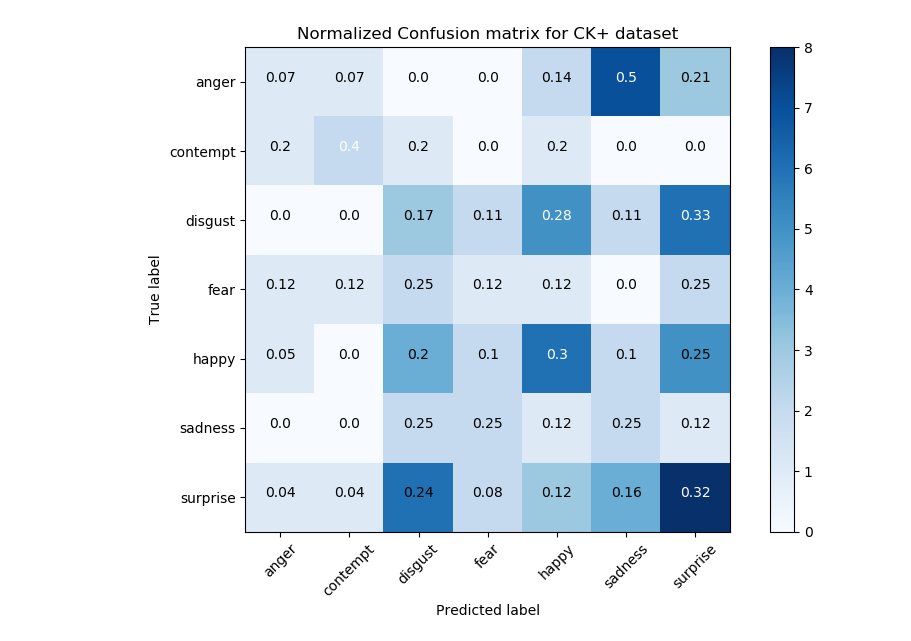
\includegraphics[width=5in]{pic/ck+_cm.png}
\caption{\,\,\,\,\,\,\,\,\,\,Confusion matrix generated from CK+ dataset testing}
\label{ck+_cm}
\end{figure}

\begin{figure}[ht]
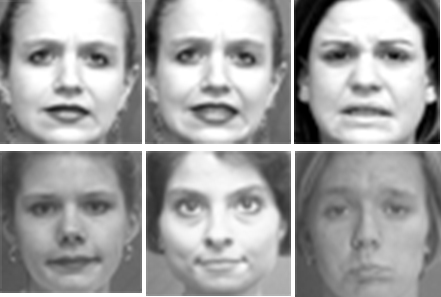
\includegraphics[width=5in]{pic/ck+similarity.jpg}
\caption{\,\,\,\,\,\,\,\,\,\,Similarity samples of contempt and fear emotion expressed in the CK+ dataset. The top horizontal faces are fear emotions and the bottom horizontal emotions are contempt emotions.}
\label{ck+_similarity}
\end{figure}

\section{Comparison with other works}
The winner of the Kaggle competition Y. Tang\cite{tang2018} achieved 69.4\% accuracy on FERC-2013 public test and 71\% accuracy on the public test with a model containing more than 7 million parameters. Sang et al.\cite{sang-2017} also achieved 71\% on FERC-2013 public test and 71.9\% on the private test with a model containing 4.19 million parameters. Arriaga et al\cite{DBLP:journals/corr/abs-1710-07557} achieved 66\% accuracy on FERC-2013 public test with a model containing approximately 600K parameters. Our proposed model contains $474K$ parameters, nevertheless, we achieved only $2\%$ lower than Y. Tang\cite{tang2018}, 2.9\% lower than Sang et al.\cite{sang-2017} and 3\% higher than O. Arriaga et al.\cite{DBLP:journals/corr/abs-1710-07557} on FERC-2013 private test. Our proposed model contains approximately 6.5 million fewer parameters compared to Y. Tang\cite{tang2018}, 4.2 million fewer parameters compared to Sang et al.\cite{sang-2017} and 126K fewer parameters compared to O. Arriaga et al.\cite{DBLP:journals/corr/abs-1710-07557}.

\begin{figure}[ht]
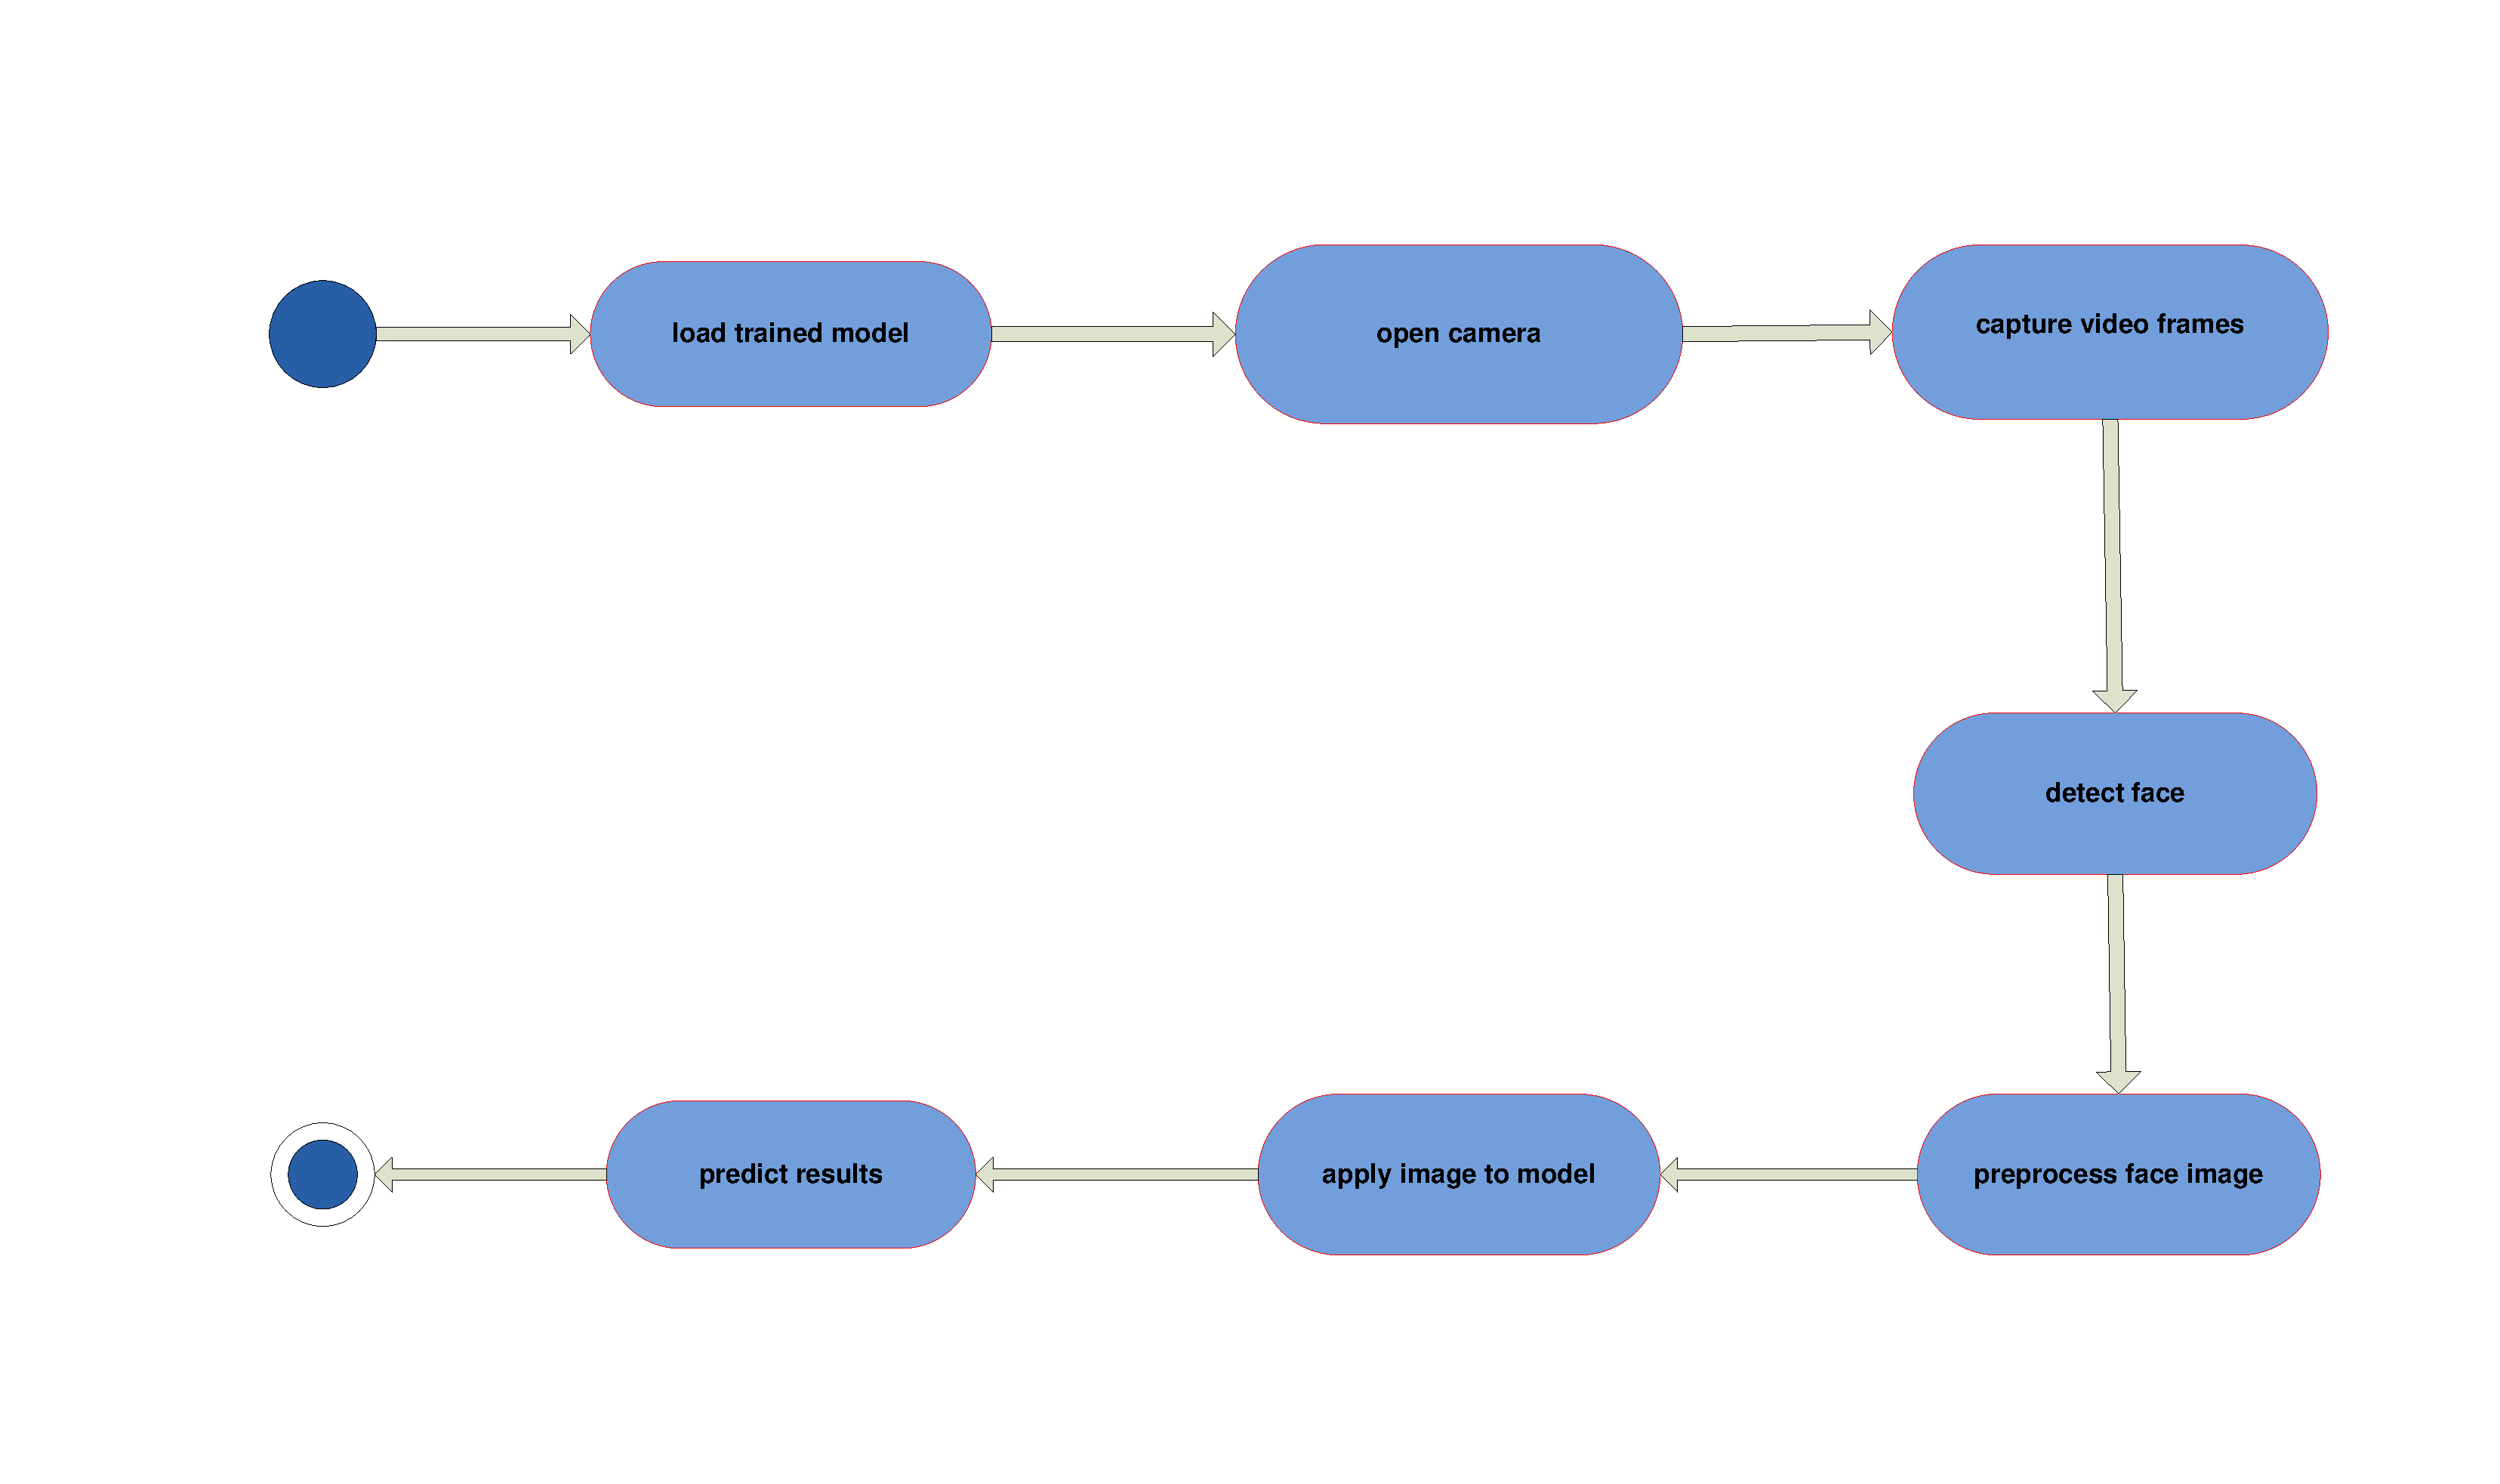
\includegraphics[width=6in]{pic/activity_diagram.pdf}
\caption{\,\,\,\,\,\,\,\,\,\,Real-time Software Activity Diagram}
\label{system_description}
\end{figure}

Duncan et al.\cite{duncan2016} achieved 62\% accuracy on JAFFE dataset with a highly parameterized CNN model containing more than 10 million parameters. Additionally, X. Chen et al.\cite{7988558} achieved 87\% accuracy on JAFFE dataset with a model containing more than 10 million parameters. However, we achieved $88\%$ accuracy on JAFFE dataset with our proposed model containing about a whooping 9 million fewer parameters compared to Duncan et al.\cite{duncan2016} and X. Chen et al.\cite{7988558}.

For CK+ dataset, Pooya et al.\cite{do_deep_7406361} achieved $96.7\%$ accuracy using quadrant pooling technique on a CNN model containing a little over 4 million parameters. Ghosh et. al. \cite{Ghosh_7344632} achieved accuracy up to $88.14\%$ using a multi-label CNN model containing only about $321K$ total parameters. However, our model outperformed the works done by both Pooya et al.\cite{do_deep_7406361} and Ghosh et. al. \cite{Ghosh_7344632} with a 99\% accuracy.

Table \ref{table_comparison} shows the comparison summary of our proposed model with other models. 

\begin{table}[ht]
% increase table row spacing, adjust to taste
\renewcommand{\arraystretch}{1.3}
\caption{\,\,\,\,\,Comparative summary with other methods}
\label{table_comparison}
\begin{center}
% The array package and the MDW tools package offers better commands
% for making tables than plain LaTeX2e's tabular which is used here.
\begin{tabular}{|c|c|c|c|c|}
\hline
Dataset & Method & No. of parameters & Accuracy \\ \hline
FERC-2013 & Y. Tang\cite{tang2018} & 7 million & 71\% \\
                 & Sang et al.\cite{sang-2017} & 4.19 million & 71.9\% \\
	      & Arriaga et al.\cite{DBLP:journals/corr/abs-1710-07557} & 600K & 66\% \\
	      & \textbf{Our method} & \textbf{474K} & \textbf{69\%} \\
\hline
JAFFE & Duncan et al.\cite{duncan2016} & 10 million & 62\% \\
                 & Chen et al.\cite{7988558} & 10 million & 87\% \\
	      & \textbf{Our method} & \textbf{474K} & \textbf{88\%} \\
\hline
CK+ & Pooya et al.\cite{do_deep_7406361} & 4 million & 96.7\% \\
                 & Ghosh et al.\cite{Ghosh_7344632} & 321K & 88.14\% \\
	      & \textbf{Our method} & \textbf{474K} & \textbf{99\%} \\
\hline
\end{tabular}
\end{center}
\end{table}

\section{Summary}
In this chapter, we presented the evaluation metrics used to measure the proposed model performance. This chapter also provides analysis of the model performance on all three datasets. Comparison of the proposed method with other state-of-the-art methods is also presented in this chapter. Finally, this chapter presents the real-time application of the proposed method. 

\begin{figure}[ht]
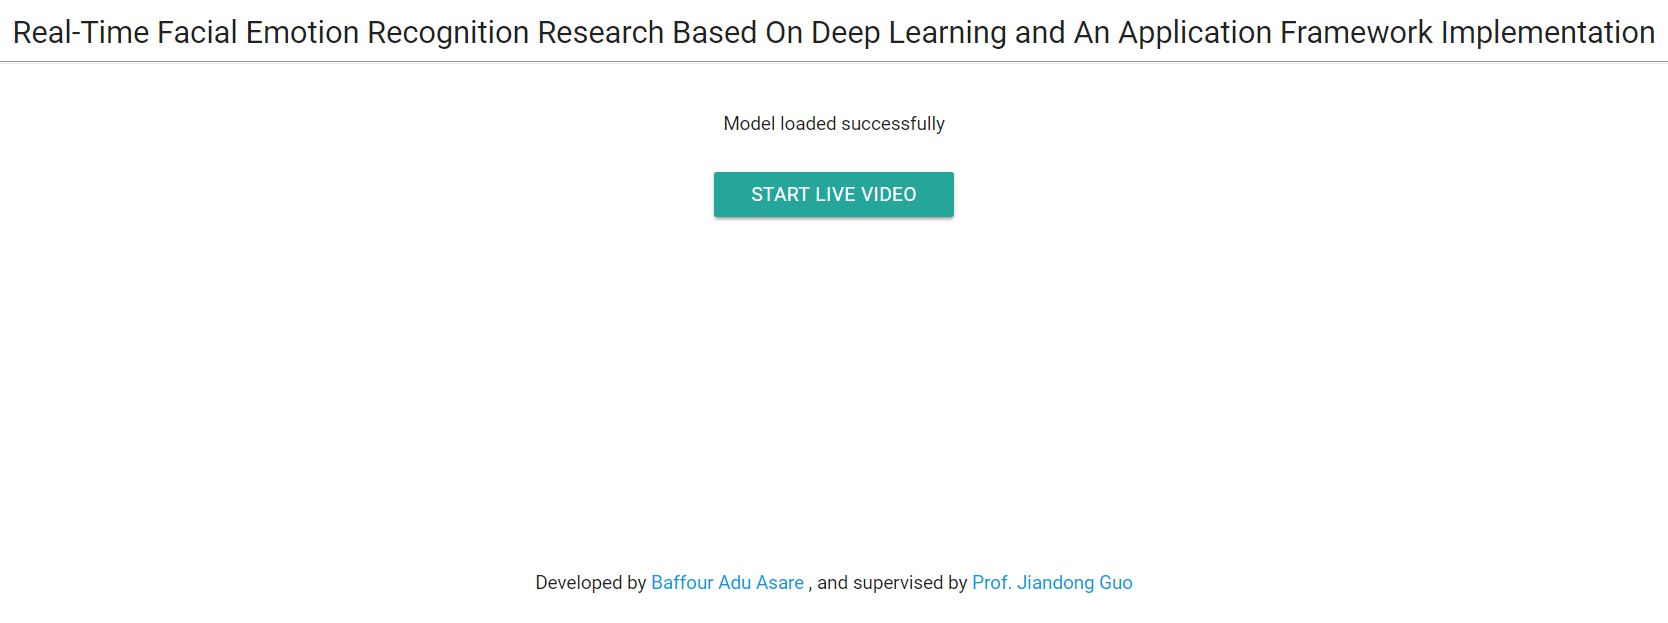
\includegraphics[width=6in]{pic/rt-interface.JPG}
\caption{\,\,\,\,\,\,\,\,\,\,Application implementation interface in web browser}
\label{rt_interface}
\end{figure}

\begin{figure}[ht]
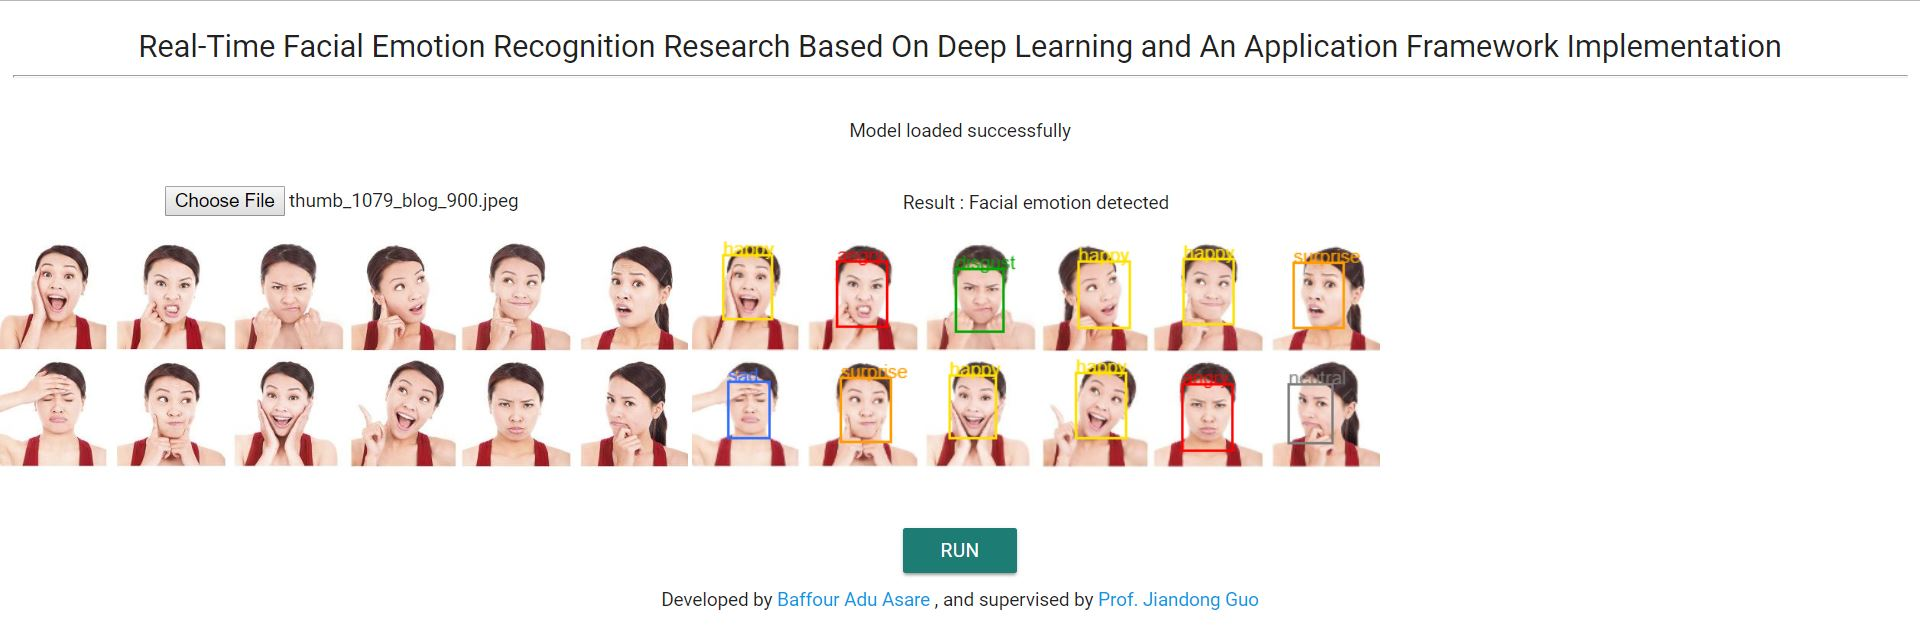
\includegraphics[width=6in]{pic/rt-1.JPG}
\caption{\,\,\,\,\,\,\,\,\,\,Application implementation showing emotion results for uploaded images in web browser}
\label{rt_uploaded}
\end{figure}

\begin{figure}[ht]
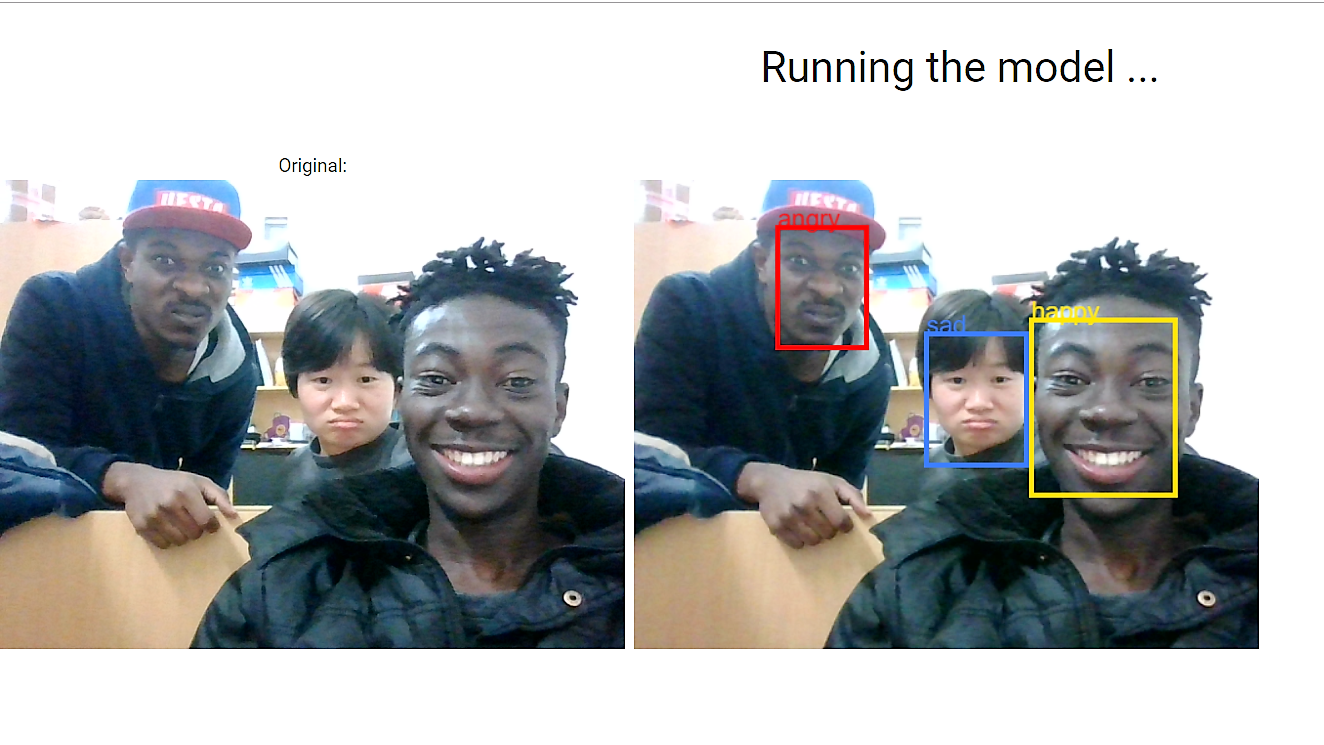
\includegraphics[width=6in]{pic/rt-2.png}
\caption{\,\,\,\,\,\,\,\,\,\,Real-time application implementation showing emotion results for multi-persons from live web cam}
\label{rt_livecam}
\end{figure}
\chapter{\,\,\,\,\,\textbf{Real-Time Implementation}}
We implement the model in two simple software systems to assess the feasibility of meeting real-time applications. Both software systems run in a web browser. The first software allows users to upload still images and outputs the emotion expressed on faces found in the image. The second software detects faces in a live web cam and predicts the facial expressions expressed on the faces. The software systems can be advanced to child care system, old age system, customer satisfactory assessment system and systems for people with hearing and speaking disorders.

\section{Application Scope and Description}
Both software systems simply take as input real-time facial expression images and recognizes the appropriate emotion expressed in the facial expression. The emotion may be \textit{Angry, Disgusted, Fear, Happy, Sad,
Surprised or Neutral}. Figure \ref{rt_uploaded} shows emotion classification from an uploaded image. This software aims to predict the facial emotion expressed with the maximum accuracy possible. The software functions are listed as follows:
\begin{enumerate}
    \item Load model
    \item Access camera
    \item Detect faces in live camera feed
    \item Send the detected face images in live camera feed to the pre-trained model
    \item Model predicts the emotion expressed in the face images
    \item Display the emotion predicted to the user
\end{enumerate}
The software activity diagram is shown in Figure \ref{system_description}. The software is made up of two main components. They are face detection component and model component.

\subsection{Application Components}
For the software system detecting emotions from uploaded images, we use used the Shape Detection API\footnote{FaceDetector: Chrome on Android, macOS, Windows 10 platfrom - https://www.chromestatus.com/feature/4757990523535360}. This API allows accessing hardware-accelerated detectors where available. For the software system detecting emotions from real-time web cam, we used the Tiny Face Detector\footnote{https://github.com/justadudewhohacks/face-api.js}. The Tiny Face Detector is a very performant, realtime face detector, which is much faster, smaller and less resource consuming compared to the SSD Mobilenet V1 face detector\footnote{A mobilenet SSD(single shot multibox detector) based face detector with pretrained model provided, powered by tensorflow object detection api, trained by WIDERFACE dataset - https://github.com/yeephycho/tensorflow-face-detection}, in return it performs slightly less well on detecting small faces.

We used \textit{TensorFlow.js converter}\footnote{https://github.com/tensorflow/tfjs-converter} to convert our Keras model to \textit{.json} file for loading and running Javascript inference. TensorFlow.js converter is an open source library to load a pretrained TensorFlow SavedModel, Frozen Model, Session Bundle or TensorFlow Hub module into the browser and run inference through TensorFlow.js. Figures \ref{} shows the web browser interface of the application.

\section{Operating Environment}
The software was ran and tested on a laptop with Windows 10, Python, Keras, CUDA (Compute Unified Device Architecture) and CuDNN (CUDA Deep Neural Netowrk) installed. The laptop must have web cam support or an external camera. The software dependencies includes:
\begin{enumerate}
    \item Tensorflow: TensorFlow is an open source software library for numerical computation using data flow graphs.
    \item Keras: High level API (Application Program Interface) designed on top of Tensorflow for fast experiment and very user-friendly.
    \item OpenCV (Open Source Computer Vision): is a library for real-time computer vision developement.
    \item Numpy: python library for numerical computations especially for multidimensional arrays.
    \item Chrome browser: To render the html pages and run javascript codes. Figure \ref{rt_interface} shows the web browser interface of the application.
    \item Chrome Shape Detection API: Provides accelerated shape detectors (e.g. human faces) for still images and/or live image feeds.
    \item face-api.js: JavaScript API for face detection and face recognition in the browser implemented on top of the tensorflow.js core API.
    \item TensorFlow.js converter: An open source library to load a pretrained TensorFlow SavedModel, Frozen Model, Session Bundle or TensorFlow Hub module into the browser and run inference through TensorFlow.js.
\end{enumerate}

\section{Functional and Non-Functional Requirements}
\subsection{Functional Requirements}
\begin{enumerate}
    \item The emotion classified feedback should be sent to the user in real-time.
    \item The system should respond to every frame captured in less than 1 second.
    \item The camera should capture frames with good quality in order to extract faces from it.
    \item The emotion classified should be accurate, i.e. correspond to the facial expression acted by the user.
    \item The computer or device running the software must have a camera and allow accessibility to the software.
\end{enumerate}
\subsection{Non-Functional Requirements}
\begin{enumerate}
    \item The camera must focus on the frontal view of the user's face in order to detect the face.
    \item The user should be expressive in the emotion.
    \item The light illumination of the user environment should be appropriate in order for efficient analysis.
\end{enumerate}
As demonstrated in Figure \ref{fig:implementation}, the software system is able to capture frames, extract faces, predict accurately and report the emotion predicted to the user.  
\begin{figure}%
\centering
\subfigure[][]{%
\label{fig:ex3-a}%
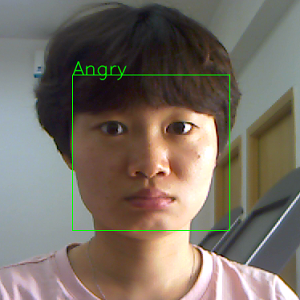
\includegraphics[height=2in]{pic/angry.png}}%
\hspace{8pt}%
\subfigure[][]{%
\label{fig:ex3-b}%
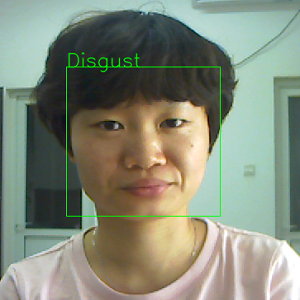
\includegraphics[height=2in]{pic/Disgust.png}} \\
\subfigure[][]{%
\label{fig:ex3-c}%
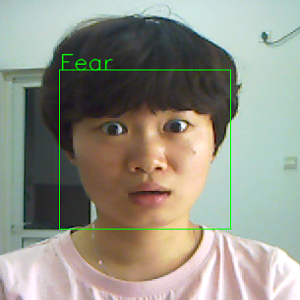
\includegraphics[height=2in]{pic/fear.png}}%
\hspace{8pt}%
\subfigure[][]{%
\label{fig:ex3-d}%
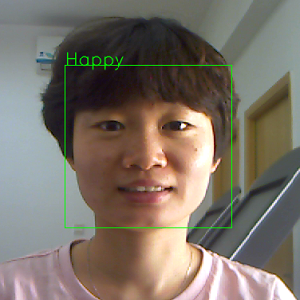
\includegraphics[height=2in]{pic/happy.png}} \\
\subfigure[][]{%
\label{fig:ex3-e}%
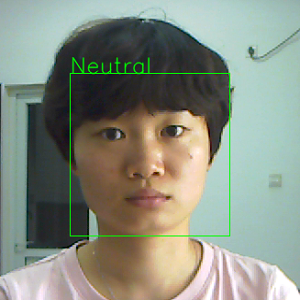
\includegraphics[height=2in]{pic/neutral.png}}%
\hspace{8pt}%
\subfigure[][]{%
\label{fig:ex3-f}%
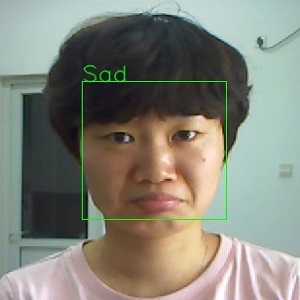
\includegraphics[height=2in]{pic/sad.jpg}} %

\caption{\,\,\,\,\,\,\,\,\,\,Real-time implementation of our model for FER on the 7 the basic emotions
\subref{fig:ex3-a} shows angry emotion;
\subref{fig:ex3-b} shows disgust emotion;
\subref{fig:ex3-c} shows fear emotion;
\subref{fig:ex3-d} shows happy emotion;
\subref{fig:ex3-e} shows neutral emotion; and
\subref{fig:ex3-f} shows sad emotion.}
\label{fig:implementation}%
\end{figure}

\section{Summary}
In this chapter, we presented the real-time application details of our proposed method. We described the the application scope and its components. We also provide the technical and non-technical requirements to ran the application successfully. Figure \ref{rt_livecam} shows real-time emotion detection in the web browser.

\chapter{\,\,\,\,\,\textbf{Conclusions}}
\section{Conclusion Remarks}
The accuracy and efficiency of CNN architectures for facial emotion recognition have very important significance to real world problems. In this thesis, we proposed a new and efficient `light weight' CNN model architecture based on depthwise separable 2D convolution for real-time emotion recognition. We implemented depthwise separable 2D convolution which reduced the network parameters drastically thereby accelerating the overall performance speed making it suitable for real-time application. We evaluated our model performance on FERC-2013 dataset provided on the Kaggle facial expression recognition competition, the Japanese Female Facial Expression (JAFFE) database and the Extended Cohn-Kanade Dataset (CK+). Our model containing only about 400K parameters achieved very competitive results of 68\% and 69\% on FERC-2013 private test and public test respectively. For JAFFE dataset, our model achieved 88\% accuracy. The model achieved an outstanding accuracy of 99\% accuracy for the CK+ dataset. Thus, we drastically reduced model complexity and eventually speed up computation. We shown that with very minimum parameters our model is a better choice over state-of-the-art models for real-time applications. Finally, as shown in Figure \ref{fig:implementation}, we demonstrated that our model can meet real-time needs by connecting a live video stream to a face detector to feed images to our trained model. The model subsequently classifies facial expressions into one of the seven emotions (Anger, Disgust, Fear, Happy, Neutral, Sad, and Surprise).

\section{Future Work}
The researches reported in this thesis have covered most important areas including the real-time application of CNN models and the accuracy improvement CNN models for facial emotion recognition. Nonetheless, due to the time limitation, there are still spaces for the future development of the real-time facial emotion recognition methods. 

A future area to be improved is to provide a mechanism to provide data for imbalance emotion classes. For example, a simple user interface can be created to allow users instantly act out imbalance emotions to be added to the dataset. In this way, the model is exposed to even more real-life data.

Another future work is to improve the model accuracy. The model sometimes confuse certain emotions for others and miss-classifies them. Hence, there is room for model accuracy improvement, even to the level of highly skilled psychologist.

Finally, we can investigate how to build a model that will be more robust for continuous emotion recognition guided by some knowledge from specific domains like psychology, social science, etc. This will make models more useful into solving specific problems.

\thesisacknowledgement
First and foremost, I would like to give thanks to Almighty God for his grace and numerous blessing and to my supervisor Prof. Jiandong Guo of the School of Information and Software Engineering at University of Electronic Science and Technology of China for his time, patience and in-depth training he gave me. Prof. Jiandong Guo and his wife have been very supportive, they have guided me immensely through out my study; in my course selections, research works and paper publication.\\
I would also like to thank all my lab mates at the Intelligent Engineering LAB (IELAB) at University of Electronic Science and Technology for their support and warm reception. Special thanks goes to Miss Li Yu Lan, who helped in the thesis real-time testing and to Mr. Wang Yao, who wrote the Chinese abstract version of the thesis.\\
Furthermore, I would like to acknowledge all professors who lectured me in my various courses. They exposed me to several research interests and laid a strong foundation for further research.\\
Finally, I must express my profound gratitude to my parents, friends and colleagues for providing me with unfailing support and continuous encouragement throughout my years of study, researching and writing this thesis. This accomplishment would not have been possible without them. \\
Thank you all.


% \thesisloadbibliography[nocite]{reference}

%
% Uncomment following codes to load bibliography database with native
% \bibliography command.
%
%\nocite{*}
\bibliographystyle{thesis-uestc}
\bibliography{reference}
%

% \thesisappendix

% Definition \pythoninline{class MyClass} means \dots
\printglossary

\thesisloadachievement{publications}

\section*{\textbf{Awards Received}}
Third Prize of Academic Achievement Award for the achievements in the field of academic research, in the academic year 2017-2018.


% \thesistranslationoriginal
% \section{A Tight Upper Bound on Bit Error Rate}


% \thesistranslationchinese

% \section{基于多载波索引键控的正交频分多路复用系统模型}

\end{document}
